\documentclass{article}

\usepackage{graphicx,psfrag}
\usepackage{graphics}
\usepackage{amsmath}
\usepackage{amsthm}
\usepackage{amsfonts}
\title{Cutoff Phenomenon  and the Mixing Property of Chaotic Maps}
\author{Tzu-Chen Liang}
\date{\today}

% End of Preamble

\newtheorem{example}{Example}
\newtheorem{assumption}{Assumption}
\newtheorem{definition}{Definition}
\newtheorem{theorem}{Theorem}
\newtheorem{lemma}{Lemma}

\begin{document}
\maketitle
%%%%%%%%%%%%%%%%%%%%%%%%%%%%%%%%%%%%%%%%%%%%%%%%%%%%%%%%%%
\begin{abstract}
We relax the definition of cutoff phenomenon discovered in finite Markov chain simulations and apply it to the study of the evolving of a probability density function under tent map and logistic map. We then prove they both present cutoffs when a sequence of initial probability densities with ascending concentration is applied. Cutoffs also observed when a simple passive scalar function is advected by the same maps with small diffusion. We refer the above two as chaotic randomizing and chaotic mixing problems, and show they are close related. Numerical evidence of cutoff is also given for 2-D standard map. 
 
\end{abstract}
%%%%%%%%%%%%%%%%%%%%%%%%%%%%%%%%%%%%%%%%%%%%%%%%%%%%%%%%%%
\section{Introduction}


\section{Background}


%%%%%%%%%%%%%%%%%%%%%%%%%%%%%%%%%%%%%%%%%%%%%%%%%%%%%%%%%%
\subsection{Measure Space and Operators}
%%%%%%%%%%%%%%%%%%%%%%%%%%%%%%%%%%%%%%%%%%%%%%%%%%%%%%%%%%
We work on the probabilistic measure space $(X,\mathcal{A},\mu)$. The transformation (or map) $S: X \rightarrow X$ is nonsingular and measurable. We choose $\mu$ to be Borel measure. In the measure space $(X,\mathcal{A},\mu)$, here are the definition of some operators,
\begin{definition} {\bfseries (Markov operator)}
Any linear operator $M:L^1 \rightarrow L^1$ satisfying 
(a) $Mf \ge 0$ for $f\ge 0, f \in L^1$; and  
(b) $||Mf|| = ||f||$ for $f\ge 0, f \in L^1$
is called a Markov operator
\end{definition} 

\begin{definition} {\bfseries (Perron-Frobenius operator)}
Let $\omega \in L^1$, for every $A \in \mathcal{A}$ the operator $P_S:L^1 \rightarrow L^1$ satisfies
  \begin{eqnarray}
    \int_A P_S \omega(x)\mu(dx) = \int_{s^{-1}(A)} \omega(x)\mu(dx)
  \end{eqnarray}
is the Perron-Frobenius operator associated with $S$.
\end{definition} 

Perron-Frobenius operator is a Markov operator. Furthermore, because our choice of measure is Borel measure. Perron-Frobenius operator can be interpreted as the operator to evolve a probability measure. Suppose the invariant measure of $S$ is $\bar{\omega}$  such that 
\begin{eqnarray}
   \bar{\omega}(S^{-1}(A)) = \bar{\omega}(A)  \mbox{    , for all } A \in \mathcal{A} 
\end{eqnarray}
we have (ommit $x$)
\begin{eqnarray}
  P_s\bar{\omega} = \bar{\omega}
\end{eqnarray}
%Suppose $S$ is invertible and since it is measure preserving, we have
% \begin{eqnarray}
% P_Sf(x) = f(S^{-1}(x)) 
% \end{eqnarray}

\begin{definition} {\bfseries (Koopman operator)}
Let $f \in L^\infty$. The operator $U_S:L^{\infty} \rightarrow L^{\infty} $ defined by 
 \begin{eqnarray}
 U_Sf(x) = f(S(x)) 
 \end{eqnarray}
is called the Koopman operator associated with $S$.
\end{definition} 

Koopman operator is adjoint to Perron-Frobenius operator, i.e. $U_S = P_S^*$ 






%%%%%%%%%%%%%%%%%%%%%%%%%%%%%%%%%%%%%%%%%%%%%%%%%%%%%%%%%%
\subsection{Cutoff Phenomenon}
%%%%%%%%%%%%%%%%%%%%%%%%%%%%%%%%%%%%%%%%%%%%%%%%%%%%%%%%%%
We also state the definition of a cutoff given by Diaconis in
\cite{Diaconis2005}. Assume that, to any finite set $\Omega$ and any
pair of probability measures $\omega$, $\bar{\omega}$ on $\Omega$ is associated
a real number $D(\omega,\bar{\omega})$ such that $D(\omega,\bar{\omega})\in [0,1]$,

\begin{eqnarray}
\max_{\Omega,\omega,\bar{\omega}} D(\omega,\bar{\omega}) = 1
\end{eqnarray}
and $D(\omega,\bar{\omega})=0$ if and only if $\bar{\omega}=\omega$. Consider a sequence of
(finite) probability spaces $(\Omega_n,\bar{\omega}_n)$, $n=1,2,...$, each
equipped with a sequence of probability measure $\omega^k_n$,
$l=0,1,...$, such that
\begin{eqnarray}
\lim_{k \rightarrow \infty} D(\omega_n,\bar{\omega}_n)=0
\end{eqnarray}
The definition of a cut-off is,

\begin{definition}
\label{cutoffdefinition}
(Diaconis) A family $(\Omega_n,\bar{\omega}_n, (\omega^k_n)_{k=0,1,...})_{n=1,2,...}$
presents a D-cut-off if there exists a sequence $(t_n)$ of positive
reals such that, for any $\epsilon \in(0,1)$,
\begin{enumerate}
  \item $\lim_{n \rightarrow \infty}D(\omega^{k_n}_n,\bar{\omega}_n) = 0 \mbox{ if }
  k_n>(1+\epsilon)t_n$
  \item $\lim_{n \rightarrow \infty}D(\omega^{k_n}_n,\bar{\omega}_n) = 1 \mbox{ if }
  k_n<(1-\epsilon)t_n $
\end{enumerate}
\end{definition}

In the next section, we need to relax the definition and set $\Omega_n$ to be infinite. We say that a family $(\Omega_n,\bar{\omega}_n, (\omega^k_n)_{k=0,1,...})_{n=1,2,...}$ presents a D-cut-off in the relaxed sense if it satisfies definition \ref{cutoffdefinition} but $\Omega_n$ is infinite. 


%%%%%%%%%%%%%%%%%%%%%%%%%%%%%%%%%%%%%%%%%%%%%%%%%%%%%%%%%%
\section{Cutoff Observed in 1-D Chaotic Map}
%%%%%%%%%%%%%%%%%%%%%%%%%%%%%%%%%%%%%%%%%%%%%%%%%%%%%%%%%%


Let $X = [0,1]$, on the measure space  $(X,\mathcal{A},\bar{\omega})$, for a given 1-D map $S: X \rightarrow X $ with $S(\bar{\omega})=\bar{\omega}$. The probability measure $\omega$  transported by $S$ in the following way, 
  \begin{eqnarray}
    \omega'(x')|dx'| = \omega(x)|dx|
  \end{eqnarray}
It is possible that there are more than one $x$ which give the same $x'$. Hence we actually have,
  \begin{eqnarray}
  \label{omegamap}
    \omega'(x') = \sum_i \left|\frac{dx_i}{dx'}\right|\omega(x) \mbox{   , for all } i \mbox{  such that  } x'=S(x_i)
  \end{eqnarray}
which is how the Perron-Frobenius operator works. In some cases we can write down the Perron-Frobenius operator explicitly, as we will see in some examples later. 


%%%%%%%%%%%%%%%%%%%%%%%%%%%%%%%%%%%%%%%%%%%%%%%%%%%%%%%%%%
\subsection{Tent Map Cutoff}
%%%%%%%%%%%%%%%%%%%%%%%%%%%%%%%%%%%%%%%%%%%%%%%%%%%%%%%%%%

\begin{figure}
\caption{\label{tentmapandlogisticmap} Tent Map and Logistic Map }
\centerline{\scalebox{0.5}[0.5]{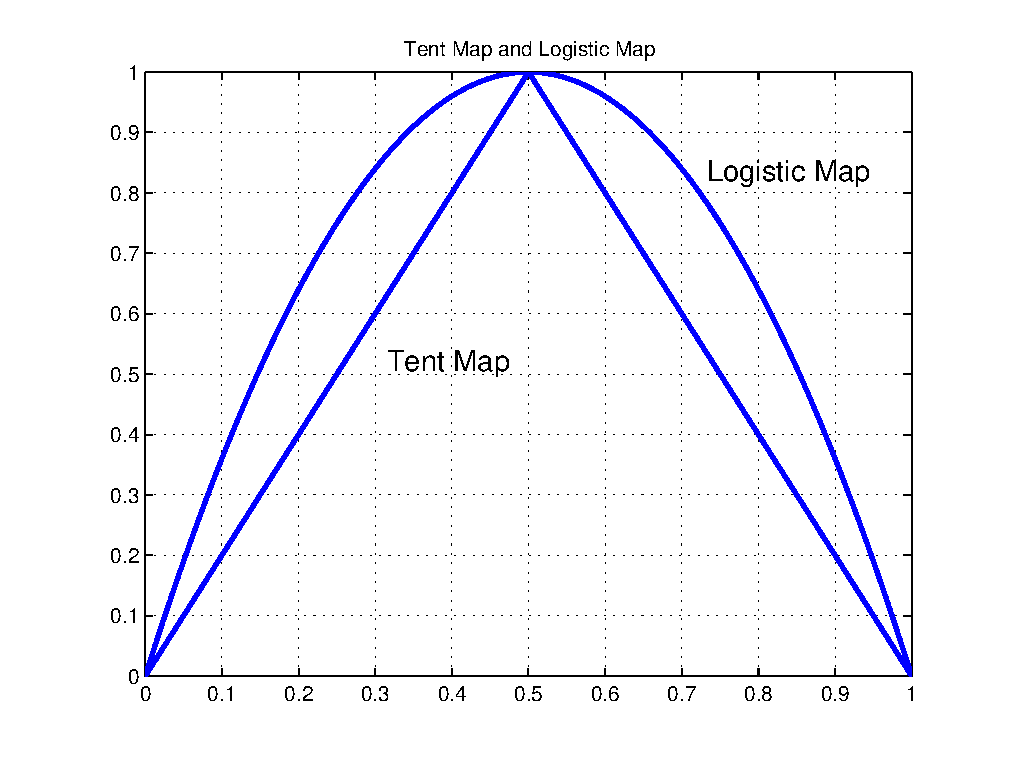
\includegraphics{tentmapandlogisticmap.eps}}}
\end{figure}


Consiter tent map,
   \begin{eqnarray}
   \label{tentmap}
     x' = S_\text{tent}(x) \equiv 1-2|x-\frac{1}{2}|
   \end{eqnarray}
with the following initial distribution on $[0 ,1]$
  \begin{eqnarray}
  \label{tentmapinitial}
    \omega_{\mu_n}^0 = \left\{ \begin{tabular}{c}
                      $\frac{1}{\mu_n}$, \mbox{  if  } $x \le \mu_n$\\ 
                      $0$, \mbox{  otherwise} 
                      \end{tabular}\right.
  \end{eqnarray}
where $\mu_1 = 1$, and $\mu_{k+1} = \frac{\mu_k}{2}$. By applying (\ref{omegamap}), the Perron-Frobenius operator of tent map is,
  \begin{eqnarray}
  \label{tentmapevolve}
    \omega_{\mu_n}^{k+1}(x) \equiv P_\text{tent} \omega_{\mu_n}^{k}(x)
                             = \frac{1}{2}\left( \omega_{\mu_n}^{k}\left(\frac{x}{2}\right)+
                                                 \omega_{\mu_n}^{k}\left(1-\frac{x}{2}\right)  \right)
  \end{eqnarray}
The invariant distribution $\bar{\omega}$ of tent map is uniform. Now consider the following sequence,
 \begin{eqnarray}
  \nu_{\mu_n}^k \equiv  |\omega_{\mu_n}^k-\bar{\omega} | 
 \end{eqnarray}
We have 
 \begin{eqnarray}
   \nu_{\mu_n}^k =  \left\{ \begin{tabular}{c} 
                    $1- 2^{1+k-n} $  ,if $k \le n-1$ \\
                    $0$   , otherwise
                    \end{tabular}\right.
 \end{eqnarray}
The of $\nu_{\mu_n}^k$ is in figure \ref{tentmapcutoff}. It clearly shows a cutoff. 

\begin{theorem} {\bfseries (Tent map cutoff)}

The family $([0,1],\bar{\omega}, (\omega^k_{\mu_n})_{k=0,1,...})_{n=1,2,...}$, where $\bar{\omega}$ is uniform in $[0,1]$ and $\omega^k_{\mu_n}$ are defined as in (\ref{tentmapinitial}) and (\ref{tentmapevolve}), presents a Total Variation-cut-off in the relaxed sense.
\end{theorem}




\begin{figure}
\caption{\label{tentmapcutoff} The plot of $\nu_{\mu_n}^k$}
\centerline{\scalebox{0.5}[0.5]{\includegraphics{tentmapcutoff.eps}}}
\end{figure}




%%%%%%%%%%%%%%%%%%%%%%%%%%%%%%%%%%%%%%%%%%%%%%%%%%%%%%%%%%
\subsection{Logistic Map Cutoff}
%%%%%%%%%%%%%%%%%%%%%%%%%%%%%%%%%%%%%%%%%%%%%%%%%%%%%%%%%%
Now let us turn to a more interesting case. Consider logistic map,  
  \begin{eqnarray}
  \label{logisticmap}
    S_\text{logistic}(x) = rx(1-x)
  \end{eqnarray}
with $r = 4$. Define initial distributions as
  \begin{eqnarray}
  \label{logisticmapinitial}
    \omega_{\mu_n}^0 = \left\{ \begin{tabular}{c}
                      $\frac{1}{\mu_n}$, \mbox{  if  } $x \le \mu_n$\\ 
                      $0$, \mbox{  otherwise} 
                      \end{tabular}\right.
  \end{eqnarray}
but now with  $\mu_0=1$, $\mu_{n+1}=\frac{1-\sqrt{1-\mu_n}}{2}$. This choice of $\omega_{\mu_n}^0$ is just to simplify the analysis and proof. Even if one chooses them as the ones we use in tent map, we would still observe cutoff. 

Again, by applying (\ref{omegamap}), we have
 \begin{eqnarray}
 \label{logisticmapevolve}
    \omega_{\mu_n}^{k+1}(x) &\equiv &P_\text{logistic} \omega_{\mu_n}^{k}(x)\\
                            &     = &\frac{1}{4\sqrt{1-x}}\left( \omega_{\mu_n}^{k}\left( \frac{1-\sqrt{1-x}}{2}\right)
                                            +\omega_{\mu_n}^{k}\left( \frac{1+\sqrt{1-x}}{2}\right) \right)
 \end{eqnarray}
The invariat distribution $\bar{\omega}$ for logistic map is 
\begin{eqnarray} 
\label{logisticmapinvariant}
 \bar{\omega} = \frac{1}{\pi\sqrt{x(1-x)}}
\end{eqnarray}
As before, we plot $\nu_{\mu_n}^k$ in figure \ref{logisticmapcutoff}.

\begin{figure}
\caption{\label{logisticmapcutoff} The plot of $\nu_{\mu_n}^k$}
\centerline{\scalebox{0.5}[0.5]{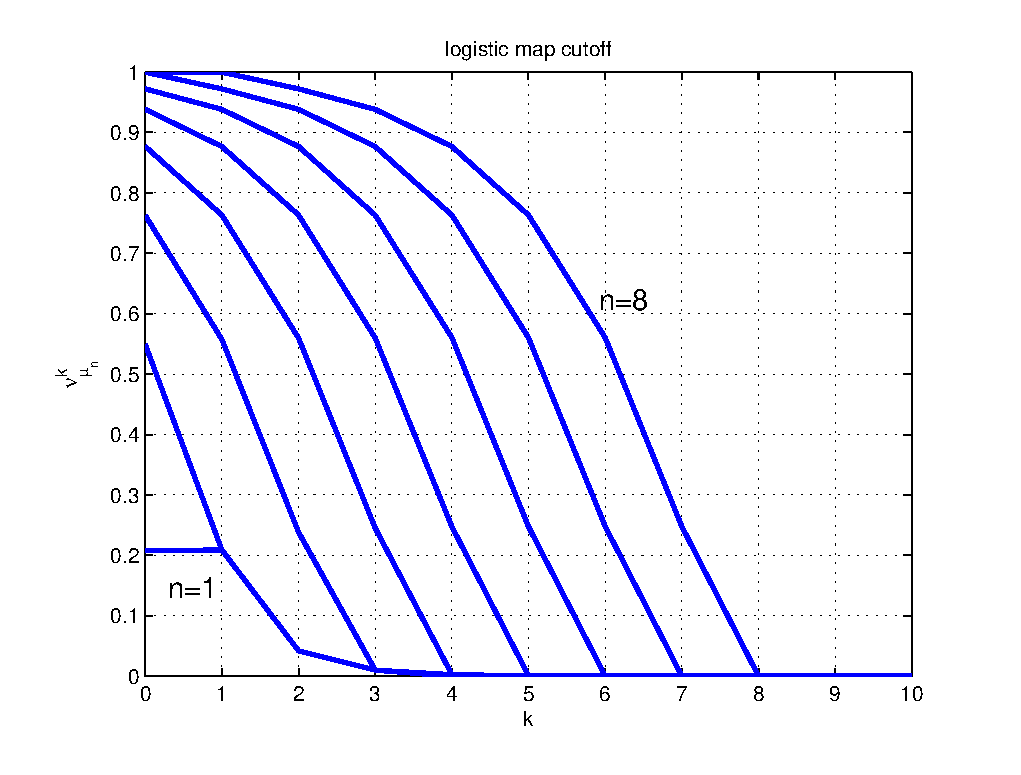
\includegraphics{logisticmapcutoff.eps}
                                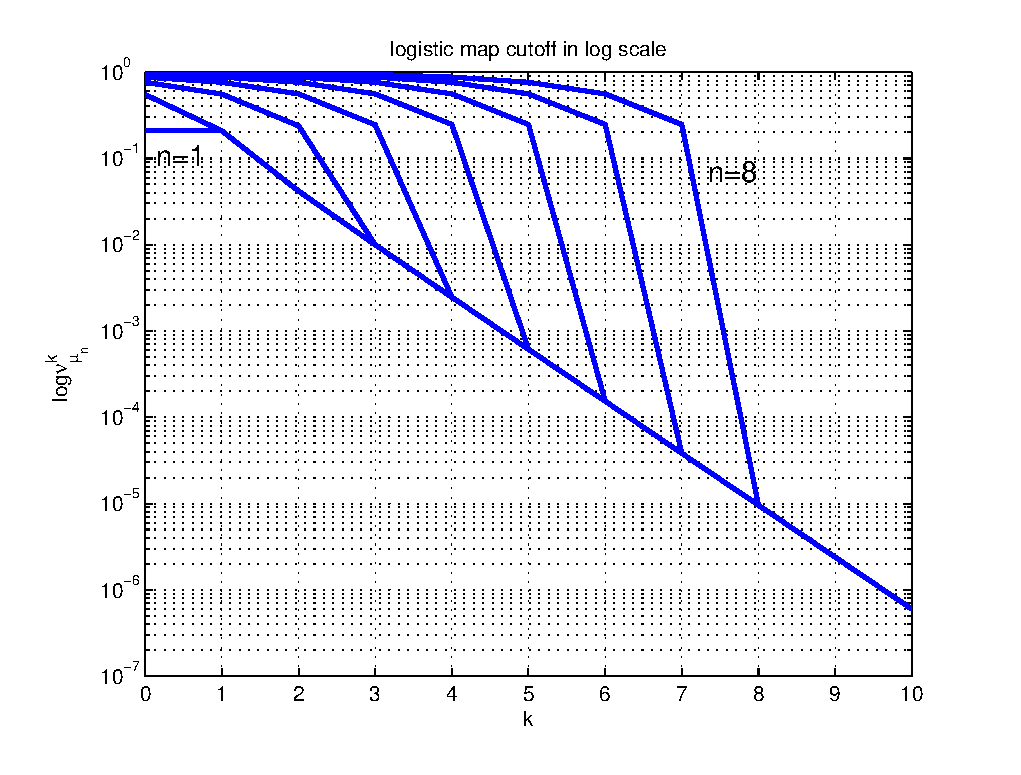
\includegraphics{logisticmapcutofflog.eps}}}
\end{figure}
The left plot in figure (\ref{logisticmapcutoff}) shows a similiar tendency as in (\ref{tentmapcutoff}). If we perform the simulation with more $n$s, the trajectories of $\nu_{\mu_n}^k$ will present a cutoff. In the log plot, one sees a more interesting thing: all the trajectories meet at some point and then decay exponentially with the same rate. 

It is well known that logistic map is equivalent to tent map by the follwoing transformation,
\begin{eqnarray} 
\label{tltransformation}
  x = \sin^2 \left(\frac{\pi y}{2}\right) \equiv T(y)
\end{eqnarray}
This means if $x$ and $y$ satisfy the above relation, then $S_\text{logistic}^k(x) = T(S_\text{tent}^k(y))$ for all $k \in \mathbb{N}$


We prove the following two lemmas.
%%%%%%%%%%%%%%%%%%%%%%%%%%%%%%%%%%%%%%%%%%%%%%%%%%%%%%%%%%
\begin{lemma}
\label{klenlemma}
When $k \ge 2$,
  \begin{eqnarray} 
     |\omega_{\mu_n}^k - \bar{\omega}|_{TV}>|\omega_{\mu_{n-1}}^{k-1} - \bar{\omega}|_{TV}
  \end{eqnarray}
for all $k \le n$ .
\end{lemma}
\paragraph{Proof} See appendix.


%%%%%%%%%%%%%%%%%%%%%%%%%%%%%%%%%%%%%%%%%%%%%%%%%%%%%%%%%%
\begin{lemma}
\label{kgenlemma}
When $n \ge 2$,
  \begin{eqnarray}
     \omega_{\mu_n}^k = \omega_{\mu_n-1}^{k}
  \end{eqnarray}
for all $k$ when $k \ge n$.
\end{lemma}
\paragraph{Proof} See appendix.



%%%%%%%%%%%%%%%%%%%%%%%%%%%%%%%%%%%%%%%%%%%%%%%%%%%%%%%%%%%
Now we have the following theorem
\begin{theorem} {\bfseries (Logistic map cutoff)}

The family $([0,1],\bar{\omega}, (\omega^k_{\mu_n})_{k=0,1,...})_{n=1,2,...}$, where $\bar{\omega}$ is defined as in (\ref{logisticmapinvariant}) and $\omega^k_{\mu_n}$ are defined as in (\ref{logisticmapinitial}) and (\ref{logisticmapevolve}), presents a Total Variation-cut-off between $k=n-1$ and $n$ in the relaxed sense .
\end{theorem}

\paragraph{Proof}
Total variation distance is non-increasing. By applying lemma \ref{klenlemma} and \ref{kgenlemma}, we obatin the theorem. 



  
%%%%%%%%%%%%%%%%%%%%%%%%%%%%%%%%%%%%%%%%%%%%%%%%%%%%%%%%%%
\subsection{Another map: $S= \sin(\pi x)$}
%%%%%%%%%%%%%%%%%%%%%%%%%%%%%%%%%%%%%%%%%%%%%%%%%%%%%%%%%%
One may suspect that lemma 2 holds for all chaotic maps similar to logistic map, but this is not true. Let us consider the following map,
 \begin{eqnarray}
    x' = \sin(\pi x)
 \end{eqnarray}
with $\mu_{n+1} = \frac{1}{\pi}\sin^{-1}(\mu_{n})$, and again $\omega_{\mu_n}^0$ is uniformly distributed in $[0, \mu_n]$ with value $\frac{1}{\mu_n}$. Figure \ref{halfsinmapcutoff} shows the $\nu_{mu_n}^k$ versus $k$ plots in normal and log scales. Clearly we do not observe the $\nu_{\mu_n}^k = \nu_{\mu_{n-1}}^{k}$ for $k \ge n$ hence lemma 2 cannot be true. However, still each trajectory shows a super-exponential decay region followed by an exponential decay region, and they presents a cutoff. In fact, we believe that cutoff happens for all chaotic map of this kind, but to prove it is not easy for most cases.  

\begin{figure}
\caption{\label{halfsinmapcutoff} The plot of $\nu_{\mu_n}^k$}
\centerline{\scalebox{0.5}[0.5]{\includegraphics{halfsinmapcutoff.eps}
                                \includegraphics{halfsinmapcutofflog.eps}}}
\end{figure}

%%%%%%%%%%%%%%%%%%%%%%%%%%%%%%%%%%%%%%%%%%%%%%%%%%%%%%%%%%
\section{Symbolic Dynamics}
%%%%%%%%%%%%%%%%%%%%%%%%%%%%%%%%%%%%%%%%%%%%%%%%%%%%%%%%%%
We would like to give and interpretation of cutoff phenomenon through symbolic dynamics.

Let $S=\{0, 1\}$ be the set of nonnegative integers consisting of $0$ and $1$. Let $\Sigma$ be the collection of all bi-infinite sequence of elements of $S$, i.e., $s\in \Sigma$ implies
 \begin{eqnarray}
 s= \{\cdots s_{-n}\cdots s_{-1}.s_0s_1\cdots s_n\cdots\}
 \end{eqnarray}
We will refer to $\Sigma$ as the space of bi-infinite sequence of two symbols. We consider a map $\sigma:\Sigma \rightarrow \Sigma$, which we shall call the shift map, defined as follows: For $s= \{\cdots s_{-n}\cdots s_{-1}.s_0\cdots s_n\cdots\}$, 
  \begin{eqnarray}
 \sigma(s)= \{\cdots s_{-n}\cdots s_{-1}s_0.s_1\cdots s_n\cdots\}
 \end{eqnarray}
There are rich results about the relation between symbolic dynamics and chaotic maps. One can read [][] for good references. Roughly speaking, one can say that given a chaotic map $S$, on its invariant set $\Lambda$, the function $\phi(x): \Lambda \rightarrow \Sigma$, which maps a point in $x\in \Lambda$ to a bi-infinite sequence, is homeomorphism. $S$ acting on $\Lambda$ and $\sigma$ acting on $\Sigma$ are topology conjugate. In other words, we have the following relation,
 \begin{eqnarray}
 S = \phi^{-1}\circ \sigma \circ \phi
 \end{eqnarray}


Since our goal is to study how the probablity density is evolved by the map and symbolic dynamics itself does not provide this information, we need to create a new object called stochastic symbol sequence. Consider $S=\{0, 1\}$ to be the symbol lists. Let $\Delta$ be the collection of all bi-infinite sequence of elements in [0,1]. We define $\delta^0 , \delta^1 \in \Delta$ for each symbol.
 \begin{eqnarray}
 \delta^0 = \{\cdots \delta_{-n}^0\cdots \delta_{-1}^0.\delta_0^0 \delta_1^0\cdots \delta_n^0\cdots\}\\
 \delta^1 = \{\cdots \delta_{-n}^1\cdots \delta_{-1}^1.\delta_0^1 \delta_1^1\cdots \delta_n^1\cdots\}
 \end{eqnarray}

The interpretation of each $\delta_i^0$ is the probability of $x$ beloning to symbol $0$. Since there are only two symbols, $\delta_i^1$ surely equals $1-\delta_i^0 $ and indicates the probability of $x$ beloning to $1$. The representation can be extended to more symbols without difficulty. However for simplicity here we only consider the two-symbol case. 

In the two-symbol case, let $\Omega\in L^\infty[\Lambda], \int_\Lambda \Omega dx=1$ denote the space of probability distribution in $\Lambda$. We want to show that there is also a homeomorphism $\psi: \Omega \rightarrow \Delta $ which maps a probability distribution $\omega(x) \in \Omega$ to the stochastic symbol sequence $\delta^0$( or $\delta^1$) uniquely. Moreover, one has
 \begin{eqnarray}
 P_s= \psi^{-1}\circ \sigma \circ \psi
 \end{eqnarray}
where $P_s$ is the Perron-Frobenius operator of $S$ and we overload the operator $\sigma$ to work on the space $\Delta$. Another important property of the function $\psi$ is for any $\omega_1, \omega_2 \in \Omega$, and $\alpha\in[0,1]$, one has,
 \begin{eqnarray}
 \label{psiislinear}
  \psi(\alpha\omega_1+(1-\alpha)\omega_2) = \alpha\psi(\omega_1)+(1-\alpha)\psi(\omega_2)
 \end{eqnarray}
where we define the convex combination of two stochastic symbol sequences are the convex combination of the individual components. This property allows us to prove some important facts later. 
 
We have successfully moved from the probability distribution $\omega(x)$ to its stochastic symbol sequence representation. Now we would like to know how total variation distance passes through, i.e., given $\omega(x)$ and $\bar{\omega}(x)$ each has stochastic symbol sequence $\{\delta^0, \delta^1\}$ and $\{\bar{\delta}^0,\bar{\delta}^1 \}$, how do we calculate $|\omega(x)-\bar{\omega}(x)|_{TV}$? It is

 \begin{eqnarray}
 \label{infiniteTV}
|\omega(x)-\bar{\omega}(x)|_{TV} = \frac{1}{2} \lim_{n \rightarrow \infty}  \sum_{s\in\Sigma} \left| \prod_{i=-n}^n\delta_i^{s_i}-\prod_{i=-n}^n\bar{\delta}_i^{s_i}  \right| 
 \end{eqnarray}

The above expression is almost impossible to evaluate due to the summation over infinity combinations. So let us consider a simpler case, when $\delta^0$ and $\bar{\delta}^0$ only have $p$ digits which are different, i.e.,$\delta_i^0 = \bar{\delta}_i^0$ when $i\in \theta$, and $|\theta| = p$. Let $\Sigma_p$ be the space of all combinations of $p$ symbol sequence with two symbols, we have,
   \begin{eqnarray}
  \label{finiteTV}
|\omega(x)-\bar{\omega}(x)|_{TV} = \frac{1}{2} \sum_{s\in\Sigma_p}  \left| \prod_{i\in \theta}\delta_i^{s_i}-\prod_{i\in\theta}\bar{\delta}_i^{s_i}  \right| 
 \end{eqnarray}
In this expression, $s$ is some finite selections of the bi-infinite symbol sequence. The important message here is that the total variation distance has nothing to do with the order: it only depends on the elements $s_i, i\in\theta$. Furthermore, (\ref{finiteTV})  can serve as a lower bound when the information besides $i\in \theta$ is unknown.  

 

The bi-infinite symbol sequence will be useful later, but before that, we would like to first consider the special case of 1-D maps, which dynamics can be respresented as the shift of a semi-infinite symbolic sequence.  

%%%%%%%%%%%%%%%%%%%%%%%%%%%%%%%%%%%%%%%%%%%%%%%%%%%%%%%%%%
\subsection{Symbolic Representation of Tent Map}
%%%%%%%%%%%%%%%%%%%%%%%%%%%%%%%%%%%%%%%%%%%%%%%%%%%%%%%%%%

 Let $\Lambda=[0, 1]$. Partition $\Lambda \cap S^{-1}_{\text{tent}}(\Lambda)$ by writing its two components as $\Lambda_1$ and $\Lambda_2$. For tenp map, $\Lambda_1=[0, 1/2]$ and $\Lambda_2=(1/2 ,1]$, we choose $\Lambda_2$ to exclude the point $1/2$ to avoid the overlap. We can associate to each $x \in \Lambda $ a sequence $s \equiv \{s_i \}_{i=0}^{\infty}$ of $0$'s and $1$'s defined by $s_i=j$ if $S_{\text{tent}}^i(x) \in \Lambda_j$. The sequence ${s_i}$ labels the iterates of $x$ according to the left-right pattern they follow. By this, we can label each $x \in \Lambda$ uniquely by a semi-infinite sequence $\phi(x)=s$ where the $s_i$'s are $0$'s and $1$'s. Let $\hat{\Sigma}$ denote the space of semi-infinite sequences of two symbols $0$'s and $1$'s. Then $\phi(x): \Lambda \rightarrow \hat{\Sigma}$ maps a point in $x\in I$ to a semi-infinite sequence. The shift operator $\sigma$ acts on $s$ by simply dropping the first entry of $s$, i.e. $\sigma(\{s_i\}_{i=0}^{\infty})=\{s_i\}_{i=1}^{\infty}$. Note this is different from how it acts on a bi-infinity sequence, and this demonstrates that the tent map "forgets" the past information. An alternative interpretation of the semi-infinite sequence is as follows: one can embed the 1-D map into a 2-D volume preserved map, and make the symbol sequence bi-infinite. However, all the $s_i$'s with $i<0$ are unobservable. We can only evaluate (and we only care about) the thing happened in the first dimension. 


Since all uni-modal maps are equivalent to tent map via transformations, the problem of evolving a specific probalibity distribution by a uni-modal map is converted to the evolving of another initial distribution by tent map. Hence we would like to derive in detail how a general initial probability distribution changes under tent map via its stochastic symbol sequence representation. Of course, we care about the total variation distance of the current distribution to the invariant distribution--uniform in tent map case. Hence use equation (\ref{finiteTV}), we have,
   \begin{eqnarray}
  \label{uniformTV}
|\omega(x)-\bar{\omega}|_{TV} = \frac{1}{2} \sum_{s\in\Sigma_p} \left| \prod_{i\in \theta}\delta_i^{s_i}-2^{-p}  \right| 
 \end{eqnarray}
In above we use the knowledge that $\delta_i^{s_i}=1/2$ for all $i$. 
The set of initial conditions defined in (\ref{tentmapinitial}) have symbol sequences as
\begin{eqnarray}
 \psi(\omega_{\mu_n}^0(x)) =  \{.\underbrace{11...1}_{n-1}\frac{1}{2}\frac{1}{2}....\}
 \end{eqnarray}
Put them into the above equation, immediately we get

   \begin{eqnarray}
  \label{uniformICTV}
   |\omega_{\mu_n}^0(x)-\bar{\omega}|_{TV} &= & \left| 1-2^{-n+1}   \right| 
 \end{eqnarray}
and follows
  \begin{eqnarray}
  \label{nunkTV}
   |\omega_{\mu_n}^k-\bar{\omega} |_{TV} =   \left\{ \begin{tabular}{c} 
                                              $1- 2^{1+k-n} $  ,if $k \le n-1$ \\
                                              $0$   , otherwise
                                             \end{tabular}\right.
  \end{eqnarray}
The $0$ comes from when $k>n-1$ the stochastic symbol sequence of $\omega_{\mu_n}^k$ is the same as $\bar{\omega}$; all the 1's are shifted and dropped. 

So by applying the stochastic symbol sequence representation, we can prove cutoff rather easily. Before we give the more general results in the next section. Let us first re-examine the logistic map case, and see how the stochastic symbol sequences can be found for this specific case. Since we are dealing with two symbol cases, let us define $\delta \equiv \delta^0$ for simplicity.

As we have discussed in the previous section, evolving (\ref{logisticmapinitial}) by logistic map is equivalent to evolving (\ref{omegamunbar0}) by tent map. Let $\delta^{\hat{\mu}_n}$ be the symbol sequence of $\omega_{\hat{\mu}_n}^0$. Clearly, we have $\delta_0^{\hat{\mu}_n}=\delta_1^{\hat{\mu}_n}=...=\delta_{n-2}^{\hat{\mu}_n}=1$. $\delta_n^{\hat{\mu}_n}$ by definition it means the follows: begin with a particle which position $x$ has the probability distribution $\omega_{\hat{\mu}_n}^0$, at the end of the $n$-th iteration, $\delta_n$ is the probability that $x \in [0,1/2]$. Note $\hat{\mu}_n = 2^{-n+1}$, we have,
\begin{eqnarray}
\label{deltan}
     \delta_{n-1}^{\hat{\mu}_n} &=&  \int_0^{\hat{\mu}/2} \omega_{\hat{\mu}_n}^0(x)dx \nonumber\\
                                &=&   \frac{1}{2+2\cos{2^{-n\pi}}}\\
     \delta_n^{\hat{\mu}_n} &=& \int_0^{\hat{\mu}/4} \omega_{\hat{\mu}_n}^0(x)dx  
                               + \int_{3\hat{\mu}/4}^{\hat{\mu}} \omega_{\hat{\mu}_n}^0(x)dx\nonumber\\
                            &=&    1-\frac{1}{2\cos(2^{-n-2}\pi)}
\end{eqnarray}
The above expressions tell us how to calculate $\delta_k^{\hat{\mu}_n}$ when $k=n$ and $k=n-1$. For $k>n$, one needs to sum up $2^{k-n+1}$ terms to get $\delta_k^{\hat{\mu}_n}$. 
%%%%%%%%%%%%%%%%%%%%%%%%%%%%%%

To simplify the notations, we define two functions $r_0$ and $r$ as
\begin{eqnarray}
  r_0(\omega(x),a,b) &=&  \int_a^b \omega(x) dx\\
  r(\omega(x),a,b)   &=&  \int_a^{a+\frac{1}{4(b-a)}} \omega(x) dx + \int_{b-\frac{1}{4(b-a)}}^b \omega(x) dx
\end{eqnarray}
then 
\begin{eqnarray}
  \delta_n^{\hat{\mu}_n} = r(\omega_{\hat{\mu}_n}^0,0,\hat{\mu}_n)
\end{eqnarray}
More generally, for $k \ge n$, 
\begin{eqnarray}
  \delta_k^{\hat{\mu}_n} = \sum_{j=0}^{k-n} r(\omega_{\hat{\mu}_n}^0,j 2^{-(k-n)} \hat{\mu}_n,(j+1) 2^{-(k-n)} \hat{\mu}_n)
\end{eqnarray}
Since $r_0(\omega_{\hat{\mu}_n}^0,0,\hat{\mu}_n)=1$, we have
\begin{eqnarray}
  \delta_k^{\hat{\mu}_n} &=& \frac{\sum_{j=0}^{k-n} r(\omega_{\hat{\mu}_n}^0,j 2^{-(k-n)} \hat{\mu}_n,(j+1) 2^{-(k-n)} \hat{\mu}_n)}
                                {r_0(\omega_{\hat{\mu}_n}^0,0,\hat{\mu}_n)} \nonumber  \\
                         &=& \frac{\sum_{j=0}^{k-n} r(\omega_{\hat{\mu}_n}^0,j 2^{-(k-n)} \hat{\mu}_n,(j+1) 2^{-(k-n)} \hat{\mu}_n)}
                                  {\sum_{j=0}^{k-n} r_0(\omega_{\hat{\mu}_n}^0,j 2^{-(k-n)} \hat{\mu}_n,(j+1) 2^{-(k-n)} \hat{\mu}_n)} 
\end{eqnarray}
Use trigonometric equalities, one can prove for all $n$ and integer $0 \le j \le k-n $,
\begin{eqnarray}
              \frac{r(\omega_{\hat{\mu}_n}^0,j 2^{-(k-n)} \hat{\mu}_n,(j+1) 2^{-(k-n)} \hat{\mu}_n)}
                   {r_0(\omega_{\hat{\mu}_n}^0,j 2^{-(k-n)} \hat{\mu}_n,(j+1) 2^{-(k-n)} \hat{\mu}_n)} =
              1-\frac{1}{2\cos(2^{-(k+2)} \pi)}
\end{eqnarray}
and is independent of $n$. From this we get the result 
\begin{eqnarray}
\label{deltashiftequality}
 \delta_{k}^{\hat{\mu}_{n}} =  1-\frac{1}{2\cos(2^{-(k+2)} \pi)}
\end{eqnarray}
and remember we have,
\begin{eqnarray}
\begin{array}{c@{{}={}}ccccc} 
 \delta^{\hat{\mu}_1} & \delta_{0}^{\hat{\mu}_1} & \delta_{1}^{\hat{\mu}_1} & \delta_{2}^{\hat{\mu}_1}& \delta_{3}^{\hat{\mu}_1}&\cdots   \\
 \delta^{\hat{\mu}_2} & 1                        & \delta_{1}^{\hat{\mu}_2} & \delta_{2}^{\hat{\mu}_2}& \delta_{3}^{\hat{\mu}_2}&\cdots   \\
 \delta^{\hat{\mu}_3} & 1                        & 1                        & \delta_{2}^{\hat{\mu}_3}& \delta_{3}^{\hat{\mu}_3}&\cdots   \\
 \delta^{\hat{\mu}_4} & 1                        & 1                        & 1                       & \delta_{3}^{\hat{\mu}_4}& \cdots  \\
   \multicolumn{6}{c}{\dotfill}
\end{array}
\end{eqnarray}
Substitute (\ref{deltashiftequality}) into above, 
\begin{eqnarray}
\begin{array}{c@{{}={}}ccccc} 
 \delta^{\hat{\mu}_1} & \delta_{0}^{\hat{\mu}_1} & \delta_{1}               & \delta_{2}              & \delta_{3}              &\cdots   \\
 \delta^{\hat{\mu}_2} & 1                        & \delta_{1}^{\hat{\mu}_2} & \delta_{2}              & \delta_{3}              &\cdots   \\
 \delta^{\hat{\mu}_3} & 1                        & 1                        & \delta_{2}^{\hat{\mu}_3}& \delta_{3}              &\cdots   \\
 \delta^{\hat{\mu}_4} & 1                        & 1                        & 1                       & \delta_{3}^{\hat{\mu}_4}& \cdots  \\
   \multicolumn{6}{c}{\dotfill}
\end{array}
\end{eqnarray}
where $\delta_i = \delta_{i}^{\hat{\mu}_i}$. whether a logistic map presents a cutoff with the initial condition (\ref{logisticmapinitial}) is completely determined by the above set of sequences.


% Because $|1-\frac{1}{2}|>|\delta^{\hat{\mu}_n}_{n-1}-\frac{1}{2}|$ and $|\delta^{\hat{\mu}_n}_{n-1}-\frac{1}{2}|> |\delta_{n-1}-\frac{1}{2}|$, we have cutoff....


%%%%%%%%%%%%%%%%%%%%%%%%%%%%%%%%%%%%%%%%%%%%%%%%%%%%%%%%%%
\subsection{General Results}
Some more general results about the total variation distance of a stochastic symbol sequence of two symbols to the uniform distribution $\bar{\omega}$, which has the representation $\bar{\delta}=\{.\frac{1}{2}\frac{1}{2}\frac{1}{2}...\}$, are given in this section. Since $\omega \mapsto |\omega-\bar{\omega}|_{TV}$ is a convex function, by using (\ref{psiislinear}) we obtain that the function $\delta \mapsto |\psi^{-1}(\delta)-\bar{\omega}|_{TV} $ is also convex, i.e., for any $\delta, \delta^* \in \Delta$, and $\alpha \in [0,1]$, we have,
 \begin{eqnarray}
\label{convexityofTV}
|\psi^{-1}(\alpha\delta+(1-\alpha)\delta^*)-\bar{\omega}|_{TV} \le 
            \alpha|\psi^{-1}(\delta)-\bar{\omega} |_{TV}+(1-\alpha)|\psi^{-1}(\delta^*)-\bar{\omega}|_{TV}
 \end{eqnarray}
So even there is no direct way to calculate the total variation distance from a stochastic symbol sequence, we can still use the convexity to deduce some useful bounds. 

We give the following lemmas:

\begin{lemma}
\label{onedifflemma}
$\delta$ and $\delta^*$ are two stochastic symbol sequences, each corresponds to the probability distribution $\omega$ and $\omega^*$, respectively. Suppose there exists a bijection $\beta: i \mapsto j$ such that $\delta_i = \delta^*_j$ for all $i\in \mathbb{Z}\setminus\{i^\dagger\}$, then
 \begin{eqnarray}
   |\delta_{i^\dagger}-\frac{1}{2}| \ge |\delta^*_{\beta(i^\dagger)}-\frac{1}{2}| \Rightarrow |\omega-\bar{\omega} |_{TV} \ge |\omega^*-\bar{\omega} |_{TV}
 \end{eqnarray}
\end{lemma}
\paragraph{Proof} $|\psi^{-1}(\delta)-\bar{\omega}|$ is independent of the order of the sequence, we can assume $\delta = \delta^*$ for all $i\in \mathbb{Z}\setminus\{i^\dagger\}$. Let $\tilde{\delta} = \delta$ for all $i\in \mathbb{Z}\setminus\{i^\dagger\}$, and $\tilde{\delta}_{i^\dagger}=1-\delta_{i^\dagger}$. Apparently, $|\psi^{-1}(\delta)-\bar{\omega}|_{TV} =|\psi^{-1}(\tilde{\delta})-\bar{\omega}|_{TV} $. When $|\delta_{i^\dagger}-\frac{1}{2}| \ge |\delta^*_{i^\dagger}-\frac{1}{2}|$, it is always possible to choose $\alpha\in[0,1]$ such that  $\delta^*_i = \alpha \delta_i +(1-\alpha) \delta^\dagger_i $. Applying (\ref{convexityofTV}) to $\delta$ and $\tilde{\delta}$ with the $\alpha$ above , we have
\begin{eqnarray}
    |\psi^{-1}(\delta^*)-\bar{\omega}|_{TV} 
                 &\le&  \alpha|\psi^{-1}(\delta)-\bar{\omega} |_{TV}+(1-\alpha)|\psi^{-1}(\tilde{\delta})-\bar{\omega}|_{TV} \nonumber\\
                 & = & |\psi^{-1}(\delta)-\bar{\omega} |_{TV}
 \end{eqnarray}

\begin{lemma}
\label{alldifflemma}
$\delta$ and $\delta^*$ are two stochastic symbol sequences, each corresponds to the probability distribution $\omega$ and $\omega^*$, respectively. Suppose there exists a bijection $\beta: i \mapsto j$ such that $|\delta_i-\frac{1}{2}| \ge |\delta^*_j-\frac{1}{2} |$ for all $i\in \mathbb{Z}$, then
 \begin{eqnarray}
   |\omega-\bar{\omega} |_{TV} \ge|\omega^*-\bar{\omega} |_{TV}
 \end{eqnarray}
\end{lemma}
\paragraph{Proof} Apply lemma \ref{onedifflemma} repeatedly. 


First we are going to generalize the lower bound result for $\delta_i=1$, for $i\in \theta$ to $\delta_i=\delta_M \le 1$. 

%%%%%%%%%%%%%%%%%%%%%%%%%%%%
\subsubsection{Lower Bound}
%%%%%%%%%%%%%%%%%%%%%%%%%%%%%
\begin{theorem}
$\delta$ and $\bar{\delta}$ are two stochastic symbol sequences, each corresponds to the probability distribution $\omega$ and the uniform distribution $\bar{\omega}$, respectively. Suppose there is a set $\theta \subset \mathbb{Z}^++\{0\} $, $|\theta|=p$ such that for all $i \in \theta$, $|\delta_i-\frac{1}{2}| \ge \epsilon$, then
\begin{eqnarray}
|\omega(x)-\bar{\omega}(x)|_{TV} \ge \mathbf{I}_{\frac{1}{2}}(p-k^*,k^*+1) - \mathbf{I}_{1-\delta^M}(p-k^*,k^*+1)
\end{eqnarray}  
where 
\begin{eqnarray}
k^* =  \left\lfloor p \frac{\log{(\frac{1}{2}-\epsilon)}-\log{(\frac{1}{2}+\epsilon})}{\log{2}+\log{(\frac{1}{2}-\epsilon)} }  \right\rfloor
\end{eqnarray}
\end{theorem}
\paragraph{proof}
Since the total variation distance is irrelevant to the order of the sequence, we can assume $\theta=\{0,1,\cdots,p-1\}$. Also, without loss of generality, we assume for $i\in \theta$, $\delta^0_i \ge \epsilon+\frac{1}{2}\equiv \delta^m$. Use equation (\ref{finiteTV}) and lemma \ref{alldifflemma}, we have
\begin{eqnarray} 
|\omega(x)-\bar{\omega}(x)|_{TV} 
                     & \ge &\frac{1}{2} \sum_{s\in\Sigma_p}  \left| \prod_{i\in \theta}\delta_i^{s_i}-\prod_{i\in\theta}\bar{\delta}_i^{s_i}  \right| \\
                     & \ge &\frac{1}{2}  \sum_{k=0}^p {p \choose k} \left|(\delta^m)^k (1-\delta^m)^{p-k} - \frac{1}{2^p} \right| \\  
                     & =   &\frac{1}{2}  \sum_{k=0}^p \left|{p \choose k} (\delta^m)^k (1-\delta^m)^{p-k} -{p \choose k} \frac{1}{2^p} \right|
\end{eqnarray} 
So the total variation distance can be lower bounded by the difference between two binomial distributions. We can find their difference by substracting their cumulative distribution functions at the point they cross over each other. So let us find the point where the first distribution is larger than the second distribution, which is to find the largest $k^*$ such that
\begin{eqnarray}
(\frac{1}{2}+\epsilon)^{k^*}(\frac{1}{2}-\epsilon)^{p-k^*}-2^{-p} \le 0
\end{eqnarray} 
so 
\begin{eqnarray}
k^* =  \left\lfloor p \frac{\log{(\frac{1}{2}-\epsilon)}-\log{(\frac{1}{2}+\epsilon})}{\log{2}+\log{(\frac{1}{2}-\epsilon)} }  \right\rfloor
\end{eqnarray}
and the CDF of a binomial distribution can be expressed in terms of the regularized incomplete beta function $\mathbf{I}$, so we have,
\begin{eqnarray}
|\omega(x)-\bar{\omega}(x)|_{TV} \ge \mathbf{I}_{\frac{1}{2}}(p-k^*,k^*+1) - \mathbf{I}_{1-\delta^M}(p-k^*,k^*+1)
\end{eqnarray}
An interesting fact of this result is when $p$ tends to $\infty$, $|\omega(x)-\bar{\omega}(x)|_{TV}$ goes to $1$ for all $\epsilon>0$. So each of these sequence of constants actually represents an eigenfunction of the map. 
%%%%%%%%%%%%%%%%%%%%%%%%%%%
\subsubsection{Upper Bound}
%%%%%%%%%%%%%%%%%%%%%%%%%%%

We have seen that for a constant sequence, the total variation distance to uniform distribution is $1$ from the previous theorem. Hence this result does not give us any information about the upper bound. We would like to bound the distance by the sum of the sequence, and give the following theorem, 
\begin{theorem}
$\delta$ and $\bar{\delta}$ are two stochastic symbol sequences, each corresponds to the probability distribution $\omega$ and the uniform distribution $\bar{\omega}$, respectively. Suppose $\sum_{i=0}^\infty |\delta_i - \frac{1}{2}| = \frac{M}{2}$, then
\begin{eqnarray}
|\omega(x)-\bar{\omega}(x)|_{TV} \le  \left\{ \begin{array}{cl}
                                   \rho - 2^{-\lceil M \rceil } &\text{ , if } \rho>1-2^{-\lceil M \rceil }\\
                                    1-2^{-\lfloor M \rfloor}    &\text{ , else}                                   \\
                                           \end{array} \right. 
\end{eqnarray}
where $\rho = \frac{1}{2} +  \frac{M-\lfloor M \rfloor}{2}$.
\end{theorem}
\paragraph{proof}
With the convixty inequality (\ref{convexityofTV}), one can show that for a set of stochastic symbol sequence $\delta^j$, $j=\{1,2,...\}$, $\sum_j{\alpha_j} = 1$
\begin{eqnarray}
 \sum_j \alpha_j|\psi^{-1}(\delta^j)-\bar{\omega}|_{TV} \ge |\psi^{-1}(\sum_j \alpha_j \delta^j)-\bar{\omega}|_{TV}
\end{eqnarray}
So for each $M$, if we can express $\delta$ as the convex combination of a set of $\delta^j$, the total variation distance $|\omega(x)-\bar{\omega}(x)|_{TV}$ can be bounded by TV of individual $\delta^j$. Let the set $\mathbf{C} = \{\delta \, | \,\sum_i|\delta_i-\frac{1}{2}|  =  \frac{M}{2}\}$. It is easy to see that $\mathbf{C} = \mathbf{conv} \mathbf{D}$, where $\mathbf{D}$ is defined as, 
\begin{eqnarray}
  \mathbf{D}=\{\delta \, | \, \delta \text{ has } \lfloor M \rfloor \text{ } 1\text{'s and one } M-\lfloor M \rfloor   \}
\end{eqnarray}
and $|\psi^{-1}(\delta)-\bar{\omega}(x)|_{TV}$ for each $\delta \in  \mathbf{D}$ can be calculated as
\begin{eqnarray}
|\psi^{-1}(\delta)-\bar{\omega}(x)|_{TV} = \left\{ \begin{array}{cl}
                                   \rho - 2^{-\lceil M \rceil } &\text{ , if } \rho>1-2^{-\lceil M \rceil }\\
                                    1-2^{-\lfloor M \rfloor}    &\text{ , else}                                   \\
                                           \end{array} \right. 
\end{eqnarray}
where $\rho = \frac{1}{2} +  \frac{M-\lfloor M \rfloor}{2}$. We obtain the upper bound by choosing the set of $\delta^j$ to be $\mathbf{D}$. 

Unfurtunately, the above upper bound is not very useful. We give another theorem
%%%%%%%%%%%%%%%%%%%%%%%%%%%%%%%%%%%%%%%%%%%%%%%%%%%%%%%%%%%%%%%%%%%%%%%%%%%%%%%%%%%%%%%%

\begin{theorem}
$\delta$ and $\bar{\delta}$ are two stochastic symbol sequences, each corresponds to the probability distribution $\omega$ and the uniform distribution $\bar{\omega}$, respectively. Suppose $\sum_{i=0}^\infty |\delta_i - \frac{1}{2}| = \frac{M}{2}$, and $\delta_i \le \delta^M$ for all $i$, then
\begin{eqnarray}
|\omega(x)-\bar{\omega}(x)|_{TV} \le  \mathbf{I}_{\frac{1}{2}}(p-k^*,k^*+1) - \mathbf{I}_{1-\delta^M}(p-k^*,k^*+1)
\end{eqnarray}
where  
\begin{eqnarray}
k^* =  \left\lfloor p \frac{\log{(\frac{1}{2}-\epsilon)}-\log{(\frac{1}{2}+\epsilon})}{\log{2}+\log{(\frac{1}{2}-\epsilon)} }  \right\rfloor
\end{eqnarray}
where $\epsilon = \delta^M - \frac{1}{2}$ and $p = \lceil \frac{M}{2\epsilon}\ \rceil$
\end{theorem}
\paragraph{proof} Combine the lower bound and upper bound proofs. 


\subsection{Random Walk on a Hypercube}
The key idea of the stochastic symbol sequences is to divide the whole sample space into two regions. The state of the particle on the corner of a $n-d$ hypercube can be represented as $x\in \mathbb{Z}^n_2$. The natural way to do this on a hypercube is by choosing anyone of its dimension $x_i$ and let state of the particle at $0$ be symbol $0$ and $1$ be symbol $1$. One should notice that it does not matter which $i$ one chooses to divide the space because of the symmetry. The beauty of this problem is once the division is done, we can calculate the stochastic symbol sequence very easily for all initial distributions. Let the particle be at the origin of a $n-d$ cube in the begining, stochastic symbol sequence of being symbol $0$ is denoted as $\delta^n = \{.\delta^n_0 \delta^n_1 \delta^n_2 \cdots  \}$. Apparently, $\delta^n_0 = 1$, but how do we calculate the rest entries of the sequences? Observe that no matter where this particle is, in the next iteration, it has the probability $\frac{n}{n+1}$ to stay the same side, and probability $\frac{1}{n+1}$ to jump to the other division. So one has
\begin{eqnarray}
   \delta^n_q &=& \delta^n_{q-1} \frac{n}{n+1} + (1-  \delta^n_{q-1}) \frac{1}{n+1} \nonumber\\
              &=&  \frac{1}{n+1} + \frac{n-1}{n+1}\delta^n_{q-1}
\end{eqnarray} 
Moreover, let $\epsilon^n_q = |\delta^n_q-\frac{1}{2}|$, we have
\begin{eqnarray}
  \epsilon^n_q =  \frac{n-1}{n+1}\epsilon^n_q
\end{eqnarray}
or 
\begin{eqnarray} 
  \epsilon^n_q =  \left(\frac{n-1}{n+1}\right)^q \epsilon^n_0
\end{eqnarray}
Hence we know all the values of the sequence. Now at $q$-th iteration, one can calculate its infinite sum, 
\begin{eqnarray} 
  \frac{M}{2} \equiv \sum_{j=q}^\infty \epsilon^n_j =  \frac{n}{2}\left( \frac{n-1}{n+1}\right)^q\\
  \delta^{n,M}_q \equiv \frac{1}{2}+ \epsilon^n_q = \frac{1}{2} +\frac{1}{2} \left(\frac{n-1}{n+1}\right)^q
\end{eqnarray}
So let $\theta=\{q,q+1,...,q+n-1\}$, we have
\begin{eqnarray}
\label{ubofrdwalk} 
|\omega_n^q(x)-\bar{\omega}(x)|_{TV} \le 
    \frac{1}{2}  \sum_{k=0}^n \left|{n \choose k} (\delta^{n,M}_q)^k (1-\delta^{n,M}_q)^{n-k} -{n \choose k} \frac{1}{2^n} \right| 
\end{eqnarray}
Then we define 
\begin{eqnarray} 
   \delta^{n,m}_q \equiv \frac{1}{2}+ \epsilon^n_{q+n} = \frac{1}{2} +\frac{1}{2} \left(\frac{n-1}{n+1}\right)^{q+n}
\end{eqnarray}
Since for $i \in \theta$, $|\delta_i-\frac{1}{2}| \ge |\delta^{n,m}_q-\frac{1}{2}| $, we have the following lower bound,
\begin{eqnarray}
\label{lbofrdwalk}  
|\omega_n^q(x)-\bar{\omega}(x)|_{TV} \ge 
    \frac{1}{2}  \sum_{k=0}^n \left|{n \choose k} (\delta^{n,m}_q)^k (1-\delta^{n,m}_q)^{n-k} -{n \choose k} \frac{1}{2^n} \right| 
\end{eqnarray}
Hence the total variation distance is bounded by equation (\ref{lbofrdwalk}) and (\ref{ubofrdwalk}). We would like to examine what happens when $n$ goes to infinity. Let $q=q(n)$, i.e., $q$ is a function of $n$ and we assume under such $q(n)$, when $n$ is large both $\delta^{n,m}_q(n)$ and $\delta^{n,M}_q(n)$ are close to $1/2$. Also both $(\epsilon^n_q)^2$  and $(\epsilon^n_{q+n})^2$ converge to $0$. We will verify these assumptions are satisfied when we get an explicit expression of $q(n)$. 

We are going to use normal distribution to replace binomial distributions in (\ref{lbofrdwalk}) and (\ref{ubofrdwalk}). Let the pdf of a normal distribution $\mathbf{N}(\mu,\sigma^2)$ be $f_{\mathbf{N}}(x;\mu,\sigma)$, and the pdf of a binomial distribution $\text{binomial}(n,p)$ be $f_b(x;n,p)$, then suppose $p$ is close to $1/2$, we have the following relation
\begin{eqnarray} 
\label{normalapprox}
 \lim_{n \rightarrow \infty}f_b(x;n,p) = f_{\mathbf{N}}(x;np,\sqrt{np(1-p)})
\end{eqnarray}
Using the above relation, we have the following,
\begin{eqnarray}
\label{normalapprox2}
 & &\lim_{n \rightarrow \infty} \frac{1}{2}\sum_{k=0}^n \left|{n \choose k} (\delta^{n,M}_{q(n)})^k 
    (1-\delta^{n,M}_{q(n)})^{n-k} -{n \choose k} \frac{1}{2^n} \right| \nonumber \\
 &=& \frac{1}{2} \int_0^x |f_{\mathbf{N}}(x;n\delta^{n,M}_{q(n)},\sqrt{n\delta^{n,M}_{q(n)}(1-\delta^{n,M}_{q(n)}}))
    -f_{\mathbf{N}}(x;\frac{n}{2},\sqrt{\frac{n}{4}}) | dx \nonumber \\
 &=& \frac{1}{2} \int_0^x |f_{\mathbf{N}}(x;\frac{n}{2}+n\epsilon_{q(n)}^n,\sqrt{\frac{n}{4}})-f_{\mathbf{N}}(x;\frac{n}{2},\sqrt{\frac{n}{4}}) | dx
\end{eqnarray}
The second equality comes from the assumption that $\lim_{n\rightarrow \infty}(\epsilon_{q(n)}^n)^2 = 0$. Equation (\ref{normalapprox2}) is just to find the total variation distance between two normal distributions with the same variance and different means. It can be carried out by using error function, so (\ref{normalapprox2}) equals
\begin{eqnarray}
 & = & \frac{1}{2}\left( 1+\text{erf}(\frac{y^*-\mu_1}{\sigma \sqrt{2}} ) \right)
                    -\frac{1}{2}\left( 1+\text{erf}(\frac{y^*-\mu_2}{\sigma \sqrt{2}} ) \right) \nonumber \\
 %& = &  \frac{1}{2} \left( \text{erf}(\frac{y^*-\mu_1}{\sigma \sqrt{2}}) -\text{erf}(\frac{y^*-\mu_2}{\sigma \sqrt{2}}) \right)\\
 & = &  \text{erf}\left(\frac{\sqrt{n}\epsilon^n_{q(n)}}{\sqrt{2}}\right)  \\
 & = &  \text{erf}\left(\frac{\sqrt{n}\left(\frac{n-1}{n+1} \right)^{q(n)}}{\sqrt{8}}\right)
\end{eqnarray}
where $\sigma = \sqrt{\frac{n}{4}}$, $\mu_1=\frac{n}{2}+n\epsilon_{q(n)}^n  $, $\mu_2 = \frac{n}{2} $ and $y^* = \frac{1}{2}(\mu_1+\mu_2)$. Hence we get an upper bound. By exactly the same derivation and replace $\epsilon_{q(n)}^n$ by $\epsilon_{q(n)+n}^n$, we can have a lower bound too. Thus, when $n$ goes to $\infty$, we have
\begin{eqnarray}
 \text{erf}\left(\frac{\sqrt{n}\left(\frac{n-1}{n+1} \right)^{q(n)+n}}{\sqrt{8}}\right) 
 \le |\omega_n^{q(n)}-\bar{\omega}|_{TV}
 \le \text{erf}\left(\frac{\sqrt{n}\left(\frac{n-1}{n+1} \right)^{q(n)}}{\sqrt{8}}\right)
\end{eqnarray}
Now we want to choose $q(n)$, which satisfies the assumptions, and to make the upper and lower bounds are independent of $n$. By notifying that $\lim_{n \rightarrow \infty} \left(\frac{n-1}{n+1} \right)^{\frac{1}{4}n\log{n}} =1/\sqrt{n} $, the obvious choice is $q(n)= \frac{1}{4}n\log{n}+cn$, and thus,
\begin{eqnarray}
 \text{erf}\left(\frac{e^{-2(c+1)}}{\sqrt{8}}\right) 
 \le |\omega_n^{\frac{1}{4}n\log{n}+cn}-\bar{\omega}|_{TV}
 \le \text{erf}\left(\frac{e^{-2c}}{\sqrt{8}}\right) 
\end{eqnarray}
which is the same as the result by Diaconis.  

%and hence the $p$ in the upper bound theorem is just $n$ and, 
%\begin{eqnarray}
%k^* =  \left\lfloor n \frac{\log{(\frac{1}{2}-\epsilon^n_q)}-\log{(\frac{1}{2}+\epsilon^n_q})}{\log{2}+\log{(\frac{1}{2}-\epsilon^n_q)} }  \right\rfloor
% \end{eqnarray}
%and 
%\begin{eqnarray}
%|\omega_n^q(x)-\bar{\omega}(x)|_{TV} \le  \mathbf{I}_{\frac{1}{2}}(n-k^*,k^*+1) - \mathbf{I}_{1-\delta^M}(n-k^*,k^*+1)
%\end{eqnarray}

%(??)And then by the lower bound theorem, we can prove the cutoff. 


%Now let us try to find where the cutoff happens. Note that the upper bound we have gets tighter and tighter when $n$ increases because $\frac{n-2}{n}$ tends to $1$. So the upper bound can serve as an approximation of the total variation distance when $n$ tends to infinity. Also, when $n$ tends to infinity, the binomial distribution can be well approximated by normal distribution, and its cdf can be expressed as error function. So let $\theta=\{q,q+1,...,q+n-1\}$, when $n\rightarrow \infty$, we have
%\begin{eqnarray}
%|\omega_n^q(x)-\bar{\omega}(x)|_{TV} 
%            &\approx& \frac{1}{2} \sum_{s\in\Sigma_n}  \left| \prod_{i\in \theta}\delta_i^{s_i}-\prod_{i\in\theta}\bar{\delta}_i^{s_i}  \right|\nonumber\\
%            & =     &\frac{1}{2}  \sum_{k=0}^n \left|{n \choose k} (\delta_M)^k (1-\delta_M)^{n-k} -{n \choose k} \frac{1}{2^n} \right|
%\end{eqnarray}
%Hence we are looking for the total vatiation of two binomial distributions: $\text{binomial}(n,\delta^M_q)$ and $\text{binomial}(n,\frac{1}{2})$. Since $\text{binomial}(n,M) \approx \mathbf{N}(n M,n M(1-M))  $, they can be approximated by normal distributions as
%\begin{eqnarray}
%\text{binomial}(n,\delta^M_q)    &\approx& \mathbf{N}\left(\left(1+\left(\frac{n-2}{n}\right)^q\right)\frac{n}{2},
%                                                    \left(1- \left(\frac{n-2}{n}\right)^{2q} \right)\frac{n}{4}\right)    \nonumber\\
%\text{binomial}(n,\frac{1}{2}) &\approx& \mathbf{N}\left(\frac{n}{2},\frac{n}{4}\right)
%\end{eqnarray}

%Now let $q \equiv q(n) = 1/4 n \log(n)+cn$ for some constant $c$, we have
%\begin{eqnarray}
%\lim_{n\rightarrow \infty}\left(\frac{n-2}{n}\right)^{2 q(n)} =0
%\end{eqnarray}
%So the difference in the variance can be neglected. Hence we need just to calculate the total variation between two identical normal distributions with different means. This can be expressed as error function, 
%\begin{eqnarray}
%|\omega_n^q(x)-\bar{\omega}(x)|_{TV} 
%           &\approx& \left|\mathbf{N}\left(\left(1+\left(\frac{n-2}{n}\right)^q\right)\frac{n}{2},\frac{n}{4}\right)-\mathbf{N}\left(\frac{n}{2},
%                           \frac{n}{4}\right)\right|_{TV} \nonumber\\
%           & = &     \frac{1}{2}\left( 1+\text{erf}(\frac{y^*-\mu_1}{\sigma \sqrt{2}} ) \right)
%                    -\frac{1}{2}\left( 1+\text{erf}(\frac{y^*-\mu_2}{\sigma \sqrt{2}} ) \right) \nonumber \\
%           & = &  \frac{1}{2} \left( \text{erf}(\frac{y^*-\mu_1}{\sigma \sqrt{2}}) -\text{erf}(\frac{y^*-\mu_2}{\sigma \sqrt{2}}) \right)
%\end{eqnarray}
%where $\sigma = \sqrt{\frac{n}{4}}$, $\mu_1= \frac{n}{2}\left(1+\left(\frac{n-2}{n}\right)^q\right) $, $\mu_2 = \frac{n}{2} $ and $y^* = \frac{1}{2}(\mu_1+%\mu_2)$, hence we get (when $n$ tends to $\infty$)
%\begin{eqnarray}
%|\omega_n^{q(n)}(x)-\bar{\omega}(x)|_{TV} 
%           \sim  \text{erf}\left( \frac{\frac{1}{\sqrt{n}}\left( \frac{n-2}{n} \right)^{1/4n \log{n}+cn}  }{\sqrt{8}} \right) 
%\end{eqnarray}
%and then $\lim_{n\rightarrow \infty}  \frac{1}{\sqrt{n}} \left( \frac{n-2}{n} \right)^{1/4n \log{n}+cn} = e^{-2c}$ gives us
%\begin{eqnarray}
%|\omega_n^{q(n)}(x)-\bar{\omega}(x)|_{TV} 
%           \sim  \text{erf}\left( \frac{e^{-2c}}{\sqrt{8}} \right) 
%\end{eqnarray}
%The result is the same as Diaconis's. 
  



\subsubsection{The equivalent condition for cutoff}

%\begin{lemma}
%For all $M \in \mathbb{Z}^+$, and the set $\theta=\{0,1,\cdots,p-1\} $, $|\theta|=p>M$, $\frac{1}{2} \sum_{s\in\Sigma_p}  \left| \prod_{i\in \theta}\delta_i^{s_i}-\prod_{i\in\theta}\bar{\delta}_i^{s_i}  \right|$ attains its maximum when 
%\begin{eqnarray} 
% \prod_i \delta^{s_i}_i<2^{-p} \Rightarrow  \prod_i \delta^{s_i}_i=0
%\end{eqnarray}
%\end{lemma}

%\paragraph{proof}
%Without loss of generality, we assume $\delta^0_i > \delta^1_i$ for all $i$. Suppose the above statement is not true, i.e., $\frac{1}{2} \sum_{s\in\Sigma_p}  \left| \prod_{i\in \theta}\delta_i^{s_i}-\prod_{i\in\theta}\bar{\delta}_i^{s_i}  \right|$ attains its maximum when $\delta^0=\hat{\delta}^{0}$, $\delta^1=\hat{\delta}^{1}$, and there is an $s = s^*$ such that $2^{-p}>\prod_i \hat{\delta}^{s^*_i}_i \neq 0$. Hence $\hat{\delta}^{s^*_i}_i \neq 0$ for all $i$, and there exists an $i^*$ such that $\hat{\delta}^{s^*_{i^*}}_{i^*}<\frac{1}{2}$. So ${s^*_{i^*}}=1$ and the pair $\{ \hat{\delta}^0_{i^*},\hat{\delta}_{i^*}^1 \} = \{\frac{1}{2}+\epsilon,\frac{1}{2}-\epsilon \}$ with some $0<\epsilon<\frac{1}{2}$. Because $M \in \mathbb{Z}^+$, It is always possible to find another two sequences $\{\tilde{\delta}^0, \tilde{\delta}^1\}$ such that $\hat{\delta}^1 = 0 \Rightarrow \tilde{\delta}^1 = 0$, $\{ \tilde{\delta}_{i^*}^0 ,\tilde{\delta}_{i^*}^1 \}=\{1,0\}$, and $\sum_{i=0}^p |\delta_i - \frac{1}{2}| = \frac{M}{2}$. Thus $|\tilde{\omega}-\bar{\omega}|>|\hat{\omega}-\bar{\omega}|$, which contradicts the assumption. 

%In the above case, the total variational distance can be calculated as
%\begin{eqnarray}
%2^{-p} \cdot |\Phi|
%\end{eqnarray}
%where $\Phi = \{\delta \in \Sigma_p| \prod_i \delta^{s_i}_i=0\}$
%%%%%%%%%%%%%%%%%%%%%%%%%%%%%%%%%%%%%%%%%%%%%%%%%%%%%%%%%%
\subsection{Short Summary}
\begin{itemize}
\item Binomial distribution proves when $n \rightarrow \infty$, for a const $\delta_i$, TV goes to $1$.
\item If for $i \le p$, $|\delta_i-\frac{1}{2}|<|\delta_M-\frac{1}{2}|$, I can get a lower bound of TV by assuming the when $i>p$, $|\delta_i-\frac{1}{2}| = 0$.
\item By knowing $\delta_i = 0.5$ for $i>p$, I can have an upper bound of TV. 
\item If $\sum_{i=0}^\infty \delta_i<\infty$, an upper bound can be obtained by letting $\delta_0= \sum_{i=0}^\infty$ and $\delta_i=0$ for all $i>0$. 
\end{itemize}

%%%%%%%%%%%%%%%%%%%%%%%%%%%%%%%%%%%%%%%%%%%%%%%%%%%%%%%%%%



%%%%%%%%%%%%%%%%%%%%%%%%%%%%%%%%%%%%%%%%%%%%%%%%%%%%%%%%%%
\section{Main Theorem}
%%%%%%%%%%%%%%%%%%%%%%%%%%%%%%%%%%%%%%%%%%%%%%%%%%%%%%%%%%




%%%%%%%%%%%%%%%%%%%%%%%%%%%%%%%%%%%%%%%%%%%%%%%%%%%%%%%%%%
%%%%%%%%%%%%%%%%%%%%%%%%%%%%%%%%%%%%%%%%%%%%%%%%%%%%%%%%%%
\section{The Cutoff Observed in Advection-Diffusion Simulation}
%%%%%%%%%%%%%%%%%%%%%%%%%%%%%%%%%%%%%%%%%%%%%%%%%%%%%%%%%%
In the above studies, we use the same map and a sequence of different initial distributions to obtain the cutoff trajectories. Now we want to extend the study of cutoff phenomenon to another sequence of simulations. In this case we study the chaotic map with small diffusion. The sequence of convergence trajectoreis will be generated by a sequence of advection-diffusion operators. 


%%%%%%%%%%%%%%%%%%%%%%%%%%%%%%%%%%%%%%%%%%%%%%%%%%%%%%%%%%
\subsection{Advection-Diffusion Operator}
%%%%%%%%%%%%%%%%%%%%%%%%%%%%%%%%%%%%%%%%%%%%%%%%%%%%%%%%%%
In the measure space $(X,\mathcal{A},\mu)$, let $P_S$ and $U_S$ be Perron-Frobenius operator and Koopman operator of map $S$. We have the following relations.
 
\vspace{0.4cm}
\begin{tabular}{l|rr}
                      & forward in time                    & backward in time     \\
\hline
        probability measure & $P_S$, $(A^T)$                       &  $P_{S^{-1}}$, $(B^T)$  \\
        function            & $P_{S^{-1}}^* = U_{S^{-1}}$, $(B)$ &  $P_S^* = U_S $, $(A)$ 
\end{tabular}
\vspace{0.4cm}

Where $U_S$, $U_{S^{-1}}$, $P_S$, and $P_{S^{-1}}$ are all real linear operators, so they can be represented by possibly infinitely dimensional Markov transient matrices $A$ and $B$ and their transposes, respectively. By the time reverse of Markov train, we also have the relation between $A$ and $B$,
  \begin{eqnarray}
  \label{ABrelation}
         B = \text{diag}(\bar{\omega}) A^T \text{diag}({\bar{\omega}}^{-1}) 
  \end{eqnarray}   
Therefore once we have obtained any one of the four operators, it is in general very easy to get the other three.  

Our goal is to find a sequence of irreducible Markov matrices $A_n$(and similarly $B_n$) which converges to $A$(and $B$). Each of the $A_n \in \mathbb{R}^{n \times n} $ represents a finite dimensional approximation of $A$. We treat the error between $A$ and $A_n$ as the added numerical diffusion so that when $n$ tends to infinity, the numerical diffusion decreases to zero. Although no matter we obtain which of them first an then apply (\ref{ABrelation}), we will have $A_n \rightarrow A$, $A_n^T \rightarrow A^T$, $B_n \rightarrow B$, and $B_n^T\rightarrow B^T$, but to approximate $A_n$ first by the definition of Koopman operator is much easier than others. To achieve this, we need a map $g_n: f(\mathbf{x}) \mapsto F $,
\begin{eqnarray}
  F_i = (g_n(f(\mathbf{x})))_i \equiv \int_{a_i} f(\mathbf{x}) d\mathbf{x}  \mbox{, for }i = 1 \mbox{ to } n
\end{eqnarray}

The sample space $X$ is discretized into regular grids and each of the grid represents one state in the new sample space. The optimal $A_n$, which has smallest error, can be found by optimal model reduction[]. However, here our goal is not to reduce the error for a specific $A_n$. Instead, we want to generate a sequence of $A_n$ with decending error(diffusion). They have to be very sparse and easy to compute so that we can go to very large $n$ and still evolve the system in moderate speed. Hence any simple first-order accruacy method can be applied. One example is the lattcice method. It approximate the map by a permutation matrix, and then adds a smoothing step to make the matrix irreducible. We create $A_n$ even simpler. Suppose $X = [0,1]$, for the map $S: X \rightarrow X$ the domain $X$ is discretized in to $n$ regular grids each with size $h$. The grids are numbered by $a_1,a_2,.., a_n$. Following the definition of Koopman operator, define the matrix $A_n$ as


 \begin{eqnarray}
 \label{Anij}
(A_n)_{ij}= \frac{\mu(S(a_i)\cap a_j)}{\mu(a_j)} 
 \end{eqnarray}

Remember that $\mu$ is Borel measure, so $(A_n)_{ij}$ is just the area ratio of $S(a_i)\cap a_j$ to $a_j$. The matrix is in general extremely sparse so we can first find the sparse pattern of it and then calculate the value of each nonzero entry. The sparse pattern of $A_n$ obtained by logistic map is shown in figure \ref{logisticmapAn}. 

We can also calculate an approximation of $A^T$ by the definition of Perron-Freobenius operator. It is,

  \begin{eqnarray}
(A_n^T)_{ij} =  \frac{\bar{\omega}(S^{-1}(a_j)\cap a_i)}{\bar{\omega}(a_i)} 
 \end{eqnarray}
where $\bar{\omega}$ is the invariant measure of $S$. Apparently the integration over a non-uniform measure is not as easy as calculating the area.   

\begin{figure}

\caption{\label{logisticmapAn} the sparse pattern of $A_n$ of logistic map for $n = 30$}
\centerline{\scalebox{0.5}[0.5]{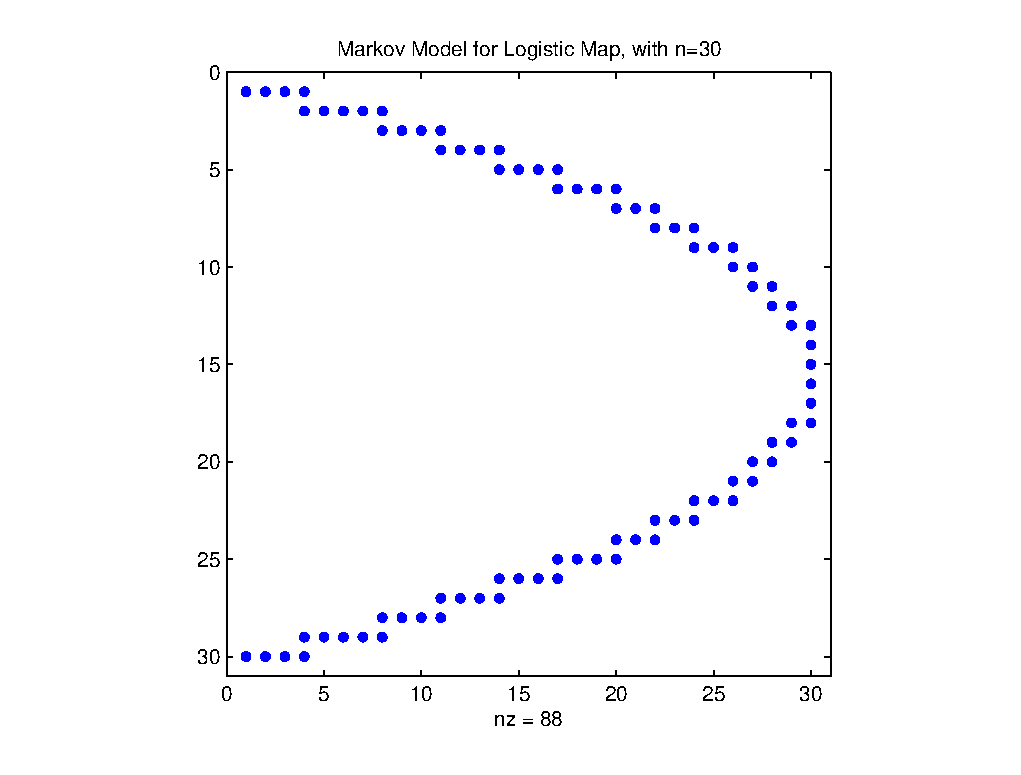
\includegraphics{logisticmapA}}}
\end{figure}


Equation (\ref{Anij}) can be extended to 2-d maps. However, in 2-d, it is already hard to decide whether $S(a_i)\cap a_j$ is non-empty, not to say calculating the areas. Hence we make the approximation procedure even simpler: suppose $X = T^2$ and $S: T^2 \rightarrow T^2$, let the grid size be $h$ on both dimensions. We number the grids by $a_1,a_2,.., a_{n^2}$. Let $\mathbf{x_i} =(x_{1i},x_{2i})$ be the center of grid $a_i$, then   
 \begin{eqnarray}
   (A_n)_{ij} =\left\{ \begin{array}{cc}
                     \frac{1}{4}, &\mbox{ if } S(x_{1i}\pm \frac{h}{2},x_{2i}\pm \frac{h}{2}) \in a_j \\
                     0,           &\mbox{ otherwise} \\
                     \end{array} \right.              
 \end{eqnarray}  
$A_n$ has only $4$ nonzeros in each row, this matrix is never explicitly formed. We need only store the size $n^2$ vector during the iteration. This approximation ensures the operation count of evolving the system is always a constant times $n$. 



 
%%%%%%%%%%%%%%%%%%%%%%%%%%%%%%%%%%%%%%%%%%%%%%%%%%%%%%%%%%
\subsection{Cutoff in $\omega_n^k$}
%%%%%%%%%%%%%%%%%%%%%%%%%%%%%%%%%%%%%%%%%%%%%%%%%%%%%%%%%%
Consider standard map,

  \begin{eqnarray}
               x_1' &=& x_1+x_2 +\epsilon \sin{2 \pi x_1} (\mbox{ mod } 1) \nonumber\\
               x_2' &=&  x_2 +\epsilon \sin{2 \pi x_1}     (\mbox{ mod } 1)
  \end{eqnarray}

Now similar to the 1-D map case, we choose vector $\omega_n^0 = [1,0,0,...,0] \in \mathbb{R}^{n^2} $ to be the initial distribution, and evolve the Markov chain by $\omega_n^{k+1} = A^T \omega_n^{k}$. For $n = 1000$ the figure \ref{demostandardmapsing} shows some of the iterations.
\begin{figure} 
\caption{\label{demostandardmapsing}}
\centerline{\scalebox{0.6}[0.6]{
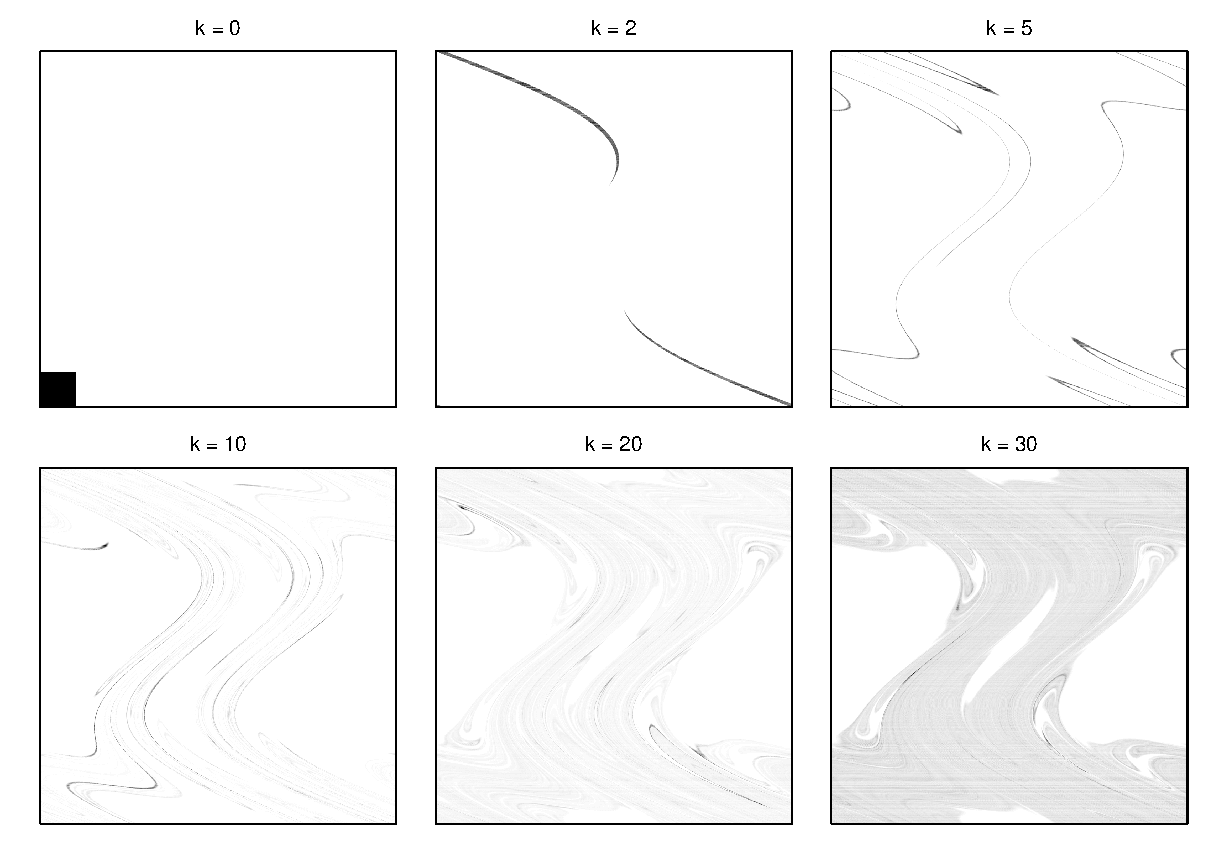
\includegraphics{demostandardmapsing.eps}
 }
}
\end{figure}
And then the cutoff figures (later)
  

%%%%%%%%%%%%%%%%%%%%%%%%%%%%%%%%%%%%%%%%%%%%%%%%%%%%%%%%%%
\subsection{Cutoff with initial condition $cos(2\pi x_2)$}
%%%%%%%%%%%%%%%%%%%%%%%%%%%%%%%%%%%%%%%%%%%%%%%%%%%%%%%%%%
The more interesting thing is that to choose $\omega_n^0 = [1,0,0,...,0]$ is not necessary for cutoff to happen. We use the following initial condition,
\begin{eqnarray}
  f_n^0 = g_n(\cos(2 \pi x_2))
\end{eqnarray}
And perform the iteration as $f_n^{k+1}= A_n f_n^k$. Selected iterations are plotted in figure \ref{demostandardmapcos}, and the trajectories of $\nu^k_n \equiv \sum_n |f^k-1|$ are shown in figure \ref{standardmapcutofftrajectory}. 

    
\begin{figure}
\caption{\label{demostandardmapcos}}
\centerline{\scalebox{0.6}[0.6]{
\includegraphics{demostandardmapcos.eps}
}}
\end{figure}


\begin{figure}
\caption{\label{standardmapcutofftrajectory}}
\centerline{
\begin{tabular}{rl}
\scalebox{0.4}[0.4]{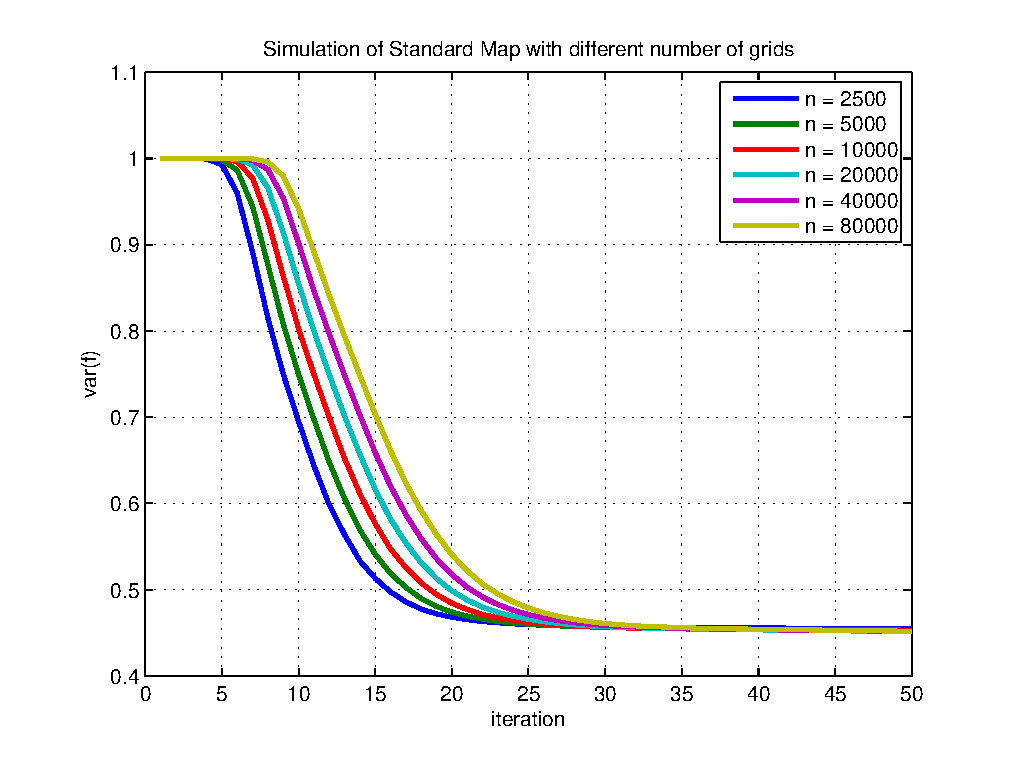
\includegraphics{standardmapcutoff}}&
\scalebox{0.4}[0.4]{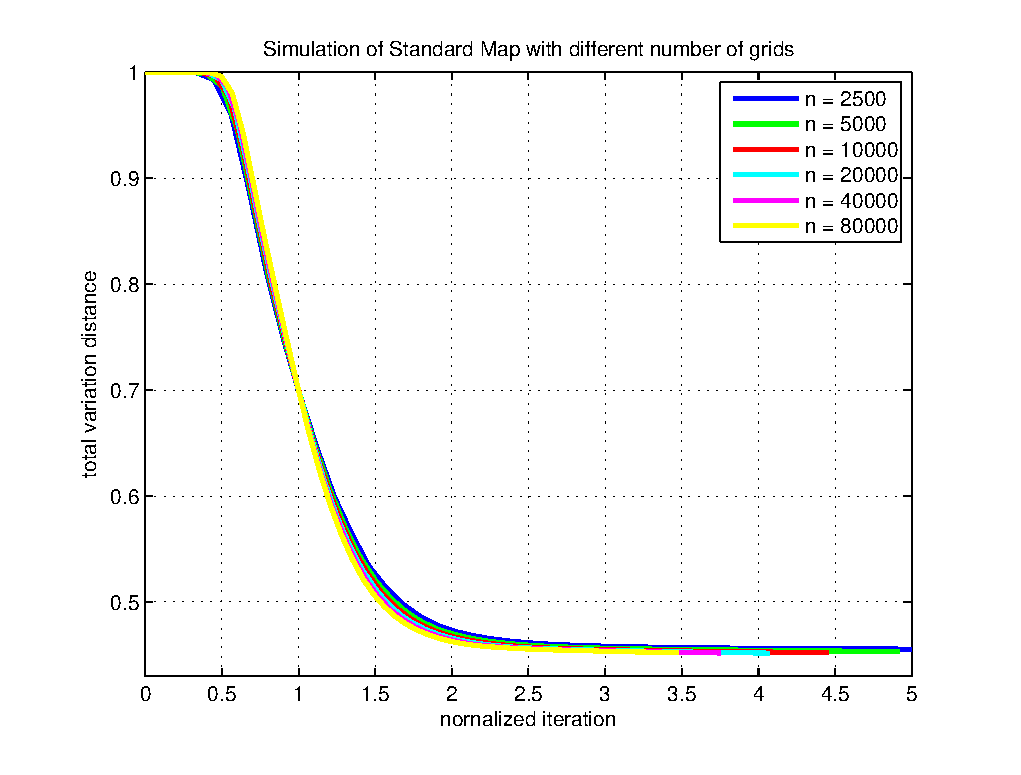
\includegraphics{standardmapcutoffn}}\\
\scalebox{0.4}[0.4]{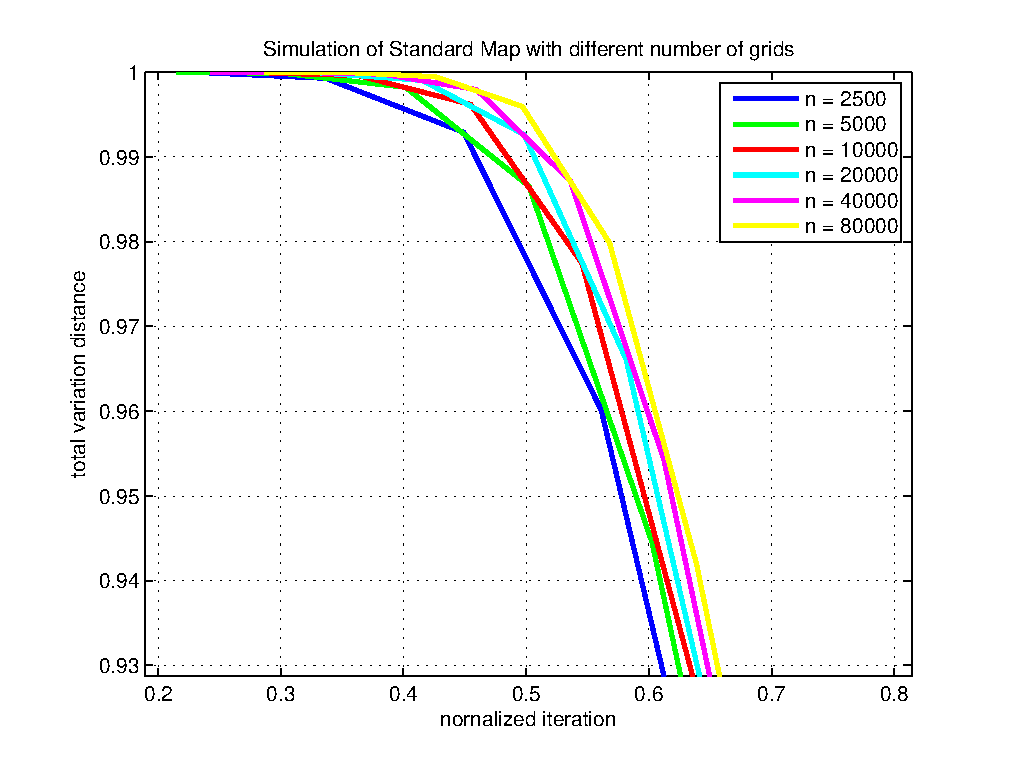
\includegraphics{standardmapcutoffmacro}}&
\scalebox{0.4}[0.4]{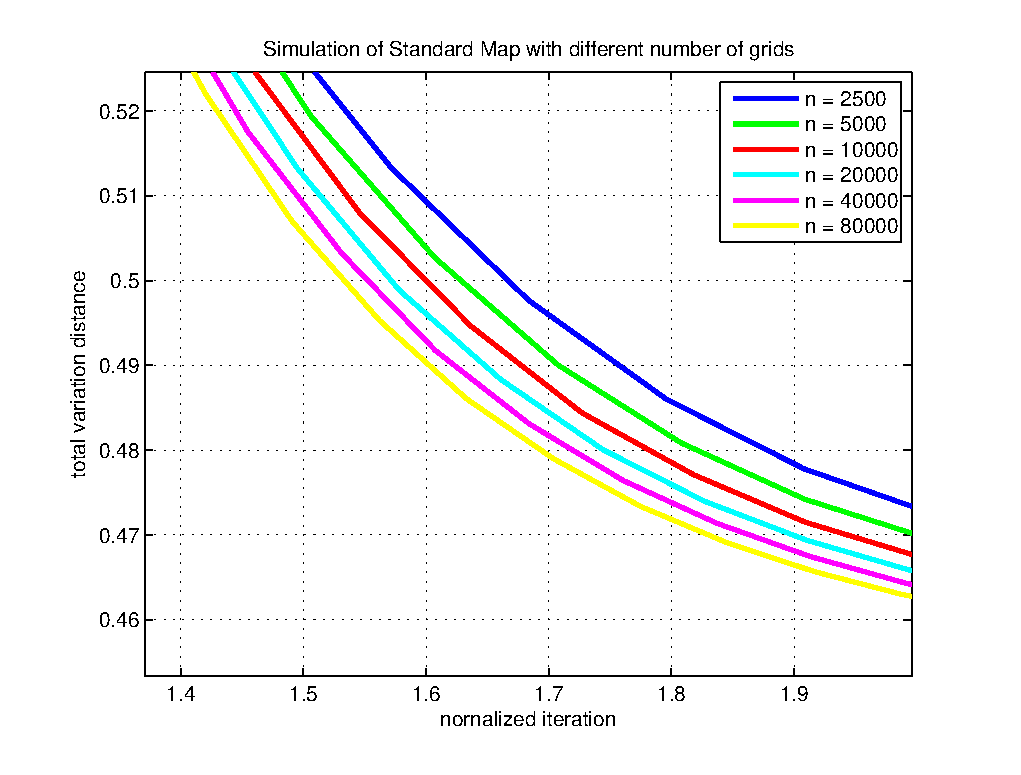
\includegraphics{standardmapcutoffmacro2}}
\end{tabular}
}
\end{figure}

%%%%%%%%%%%%%%%%%%%%%%%%%%%%%%%%%%%%%%%%%%%%%%%%%%%%%%%%%%
%%%%%%%%%%%%%%%%%%%%%%%%%%%%%%%%%%%%%%%%%%%%%%%%%%%%%%%%%%
%\section{Cutoff of functions}
%%%%%%%%%%%%%%%%%%%%%%%%%%%%%%%%%%%%%%%%%%%%%%%%%%%%%%%%%%
%%%%%%%%%%%%%%%%%%%%%%%%%%%%%%%%%%%%%%%%%%%%%%%%%%%%%%%%%%
%%%%%%%%%%%%%%%%%%%%%%%%%%%%%%%%%%%%%%%%%%%%%%%%%%%%%%%%%%
%\subsection{Continuous Version}
%%%%%%%%%%%%%%%%%%%%%%%%%%%%%%%%%%%%%%%%%%%%%%%%%%%%%%%%%%
%In the measure space $(X,\mathcal{A},\mu)$, for the map $S$, $P_S$ and $U_S$ denote its Perron-Frobenius and Koopman operators, respectively. Suppose for any sequence of sets $B_n \subset X$, such that $B_0 \supset B_1 \supset...$, and $\lim_{n \rightarrow \infty} \mu(B_n)=0$, The family $(X,\bar{\omega}, (\omega^k_n)_{k=0,1,...})_{n=1,2,...}$ presents a cutoff at $k=h(n)$, where $\bar{\omega}$ is the invariant measure of $S$, $\omega^{k+1}_n = P_S \omega^{k+1}_n$ and 
%  \begin{eqnarray}
%  \label{logisticmapinitial}
%    \omega_n^0(\mathbf{x}) = \left\{ \begin{tabular}{cl}
%                      $\frac{1}{\mu(B_n)}$&, \mbox{  if  } $\mathbf{x} \in B_n$\\ 
%                      $0$&, \mbox{  otherwise} 
%                      \end{tabular}\right.
%  \end{eqnarray}


%%%%%%%%%%%%%%%%%%%%%%%%%%%%%%%%%%%%%%%%%%%%%%%%%%%%%%%%%%
%\subsection{Discrete Version}
%%%%%%%%%%%%%%%%%%%%%%%%%%%%%%%%%%%%%%%%%%%%%%%%%%%%%%%%%%
%From the relations
%\begin{eqnarray}
% \omega_n^{k+1} &=& A_n^T \omega_n^{k} \nonumber \\
%  f_n^{k}       &=& A_n  f_n^{k+1}
%\end{eqnarray}
%We have
%\begin{eqnarray}
% (\omega_n^{k+1})^T f_n^{k+1}= (\omega_n^{k})^T f_n^{k} \mbox{     , for all } k   
%\end{eqnarray}

%Now consier $\omega_n^k = \omega_{\mu_n}^k$, where
%  \begin{eqnarray}
%  \label{logisticmapinitial}
%    \omega_{\mu_n}^0 = \left\{ \begin{tabular}{cl}
%                      $\frac{1}{\mu_n}$&, \mbox{  if  } $x \in [x_0, x_0+\mu_n]$\\ 
%                      $0$&, \mbox{  otherwise} 
%                      \end{tabular}\right.
%  \end{eqnarray}
%and $1 \ge \mu_0 >  \mu_{1} > ... > \mu_{k}>...$. Suppose the sequence of Markov chain $A_n$ persents a cutoff at $h(n)$ with initial distributions $\omega_{\mu_n}^0$ for all $x_0\in[0,1-\mu_n]$, then at iteration $k=h(n)+ \Delta_n$, $\omega_{\mu_n}^{h(n)+ \Delta_n} $ is non-vanishing everywhere. Becasue for any function $f_n^{h(n)+ \Delta_n}$, $(\omega_{\mu_n}^0)^T f_n^0 = (\omega_{\mu_n}^{h(n)+ \Delta_n})^T f_n^{h(n)+ \Delta_n} $




\begin{figure}
\caption{\label{cutoffexplain}}
\centerline{\scalebox{0.6}[0.6]{
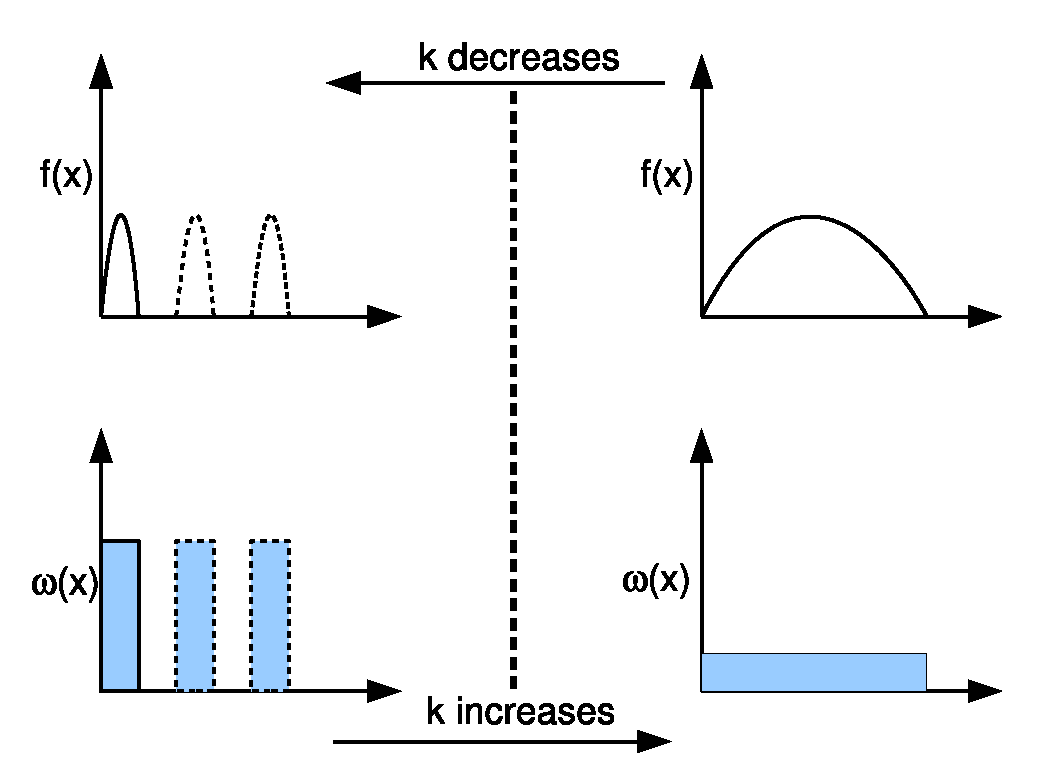
\includegraphics[trim=1cm 1cm 1cm 1cm]{cutoffexplain.eps}
}}
\end{figure}

%%%%%%%%%%%%%%%%%%%%%%%%%%%%%%%%%%%%%%%%%%%%%%%%%%%%%%%%%%
%%%%%%%%%%%%%%%%%%%%%%%%%%%%%%%%%%%%%%%%%%%%%%%%%%%%%%%%%%
%\section{Define the Degree of Chaos through Cutoff}
%%%%%%%%%%%%%%%%%%%%%%%%%%%%%%%%%%%%%%%%%%%%%%%%%%%%%%%%%%
%%%%%%%%%%%%%%%%%%%%%%%%%%%%%%%%%%%%%%%%%%%%%%%%%%%%%%%%%%
%\subsection{Degree of Chaos}
%%%%%%%%%%%%%%%%%%%%%%%%%%%%%%%%%%%%%%%%%%%%%%%%%%%%%%%%%%
%Do decide a map is chaotic and tell how chaotic it is is a hard question. In general, the degree of chaos can be divided into the following categories. 
%\begin{definition} {\bfseries (Ergodic)}
%$S$ is called ergodic if every invariant set $A\in \mathcal{A}$ is such that $\mu(A)=0$ or $\mu(X \setminus A)=0$
%\end{definition}
%\begin{definition} {\bfseries (Mixing)}
%If 
% \begin{eqnarray}
%  \lim_{n \rightarrow \infty} \mu(A \cup S^{-n}(B))  = \mu(A) \mu(B) \mbox{   ,for all } A, B \in \mathcal{A}
% \end{eqnarray}
%then $S$ is called mixing.  
%\end{definition}
%\begin{definition} {\bfseries (Exact)}
%If  
% \begin{eqnarray}
%  \lim_{n \rightarrow \infty} \mu(S^n(A))  =1 \mbox{   ,for all } A \in \mathcal{A}
% \end{eqnarray}
%then $S$ is called exact. 
%\end{definition}

%Exactness implies mixing, and mixing implies ergodic. Hence one may feel that by telling a map belonging to which of these three catogries, we can tell how chaotic it is. However, this is in general not very informative in telling us how fast this chaotic map mixes a certain function. The three 1-D maps we have studied in section 1 are all exact maps, and standard map we studied in the previous section is not even ergodic. 

%Hence we suggest to define the mixing property of a chaotic map through the cutoff trajectories of its advection-diffusion operator. Here are the observations:
%\begin{itemize}
%\item If the map is ergodic but not mixing, the diffusion part in the operator works just like the normal diffusion, and we will not see cutoffs. (cutoff at $k=\infty$)
%\item If the map is mixing but not exact, the diffusion part in the operator is enhanced by the advection part, and we will see cutoffs.
%\item If the map is exact, then the exact perron-frobenius operator $A^T$ is already diffusive. This effect works in the same(or larger or smaller?) scale as the added diffusion in $A_n^T$. They are both enhanced by the advection part of the operator, hence we will see cutoff. 
%\end{itemize} 

%It is possible that a set $A \subset X$ is an invariant set of $S$, and $S$ on $A$ and on $X\backslash A$ belong to different catogaries of the chaotic %degrees. This will again reflects in the cutoff trajectories of $A_n$   


\section{Conclusion}
We prove that tent map and logistic map both present cutoffs when suitable sequence of initial probability distributions are chosen. We also numerically demonstrate that a similar cutoff can be observed when a passive scalar function is advected by the chaotic map with small diffusion. The above two findings show that phase change appears in both chaotic randomizing and chaotic mixing problems. 



%%%%%%%%%%%%%%%%%%%%%%%%%%%%%%%%%%%%%%%%%%%%%%%%%%%%%%%%%%
%%%%%%%%%%%%%%%%%%%%%%%%%%%%%%%%%%%%%%%%%%%%%%%%%%%%%%%%%%
\section{Appendix}
Here are the small lemmas I need.

proof of lemma \ref{klenlemma}
\paragraph{Proof}
Let $p_{\mu_n}^k$ be the point such that $\omega_{\mu_n}^k(p_{\mu_n}^k) = \bar{\omega}(p_{\mu_n}^k)$. By lemmas, we have  $p_{\mu_n}^k < p_{\mu_{n-1}}^{k-1}$, and $\omega_{\mu_n}^k(x)< \omega_{\mu_{n-1}}^{k-1}(x)$ for $x< p_{\mu_n}^k $, Let
 \begin{eqnarray}
  \Delta =  \int_0^{p_{\mu_{n-1}}^{k-1}} \omega_{\mu_{n-1}}^{k-1}(x) -\omega_{\mu_n}^k(x) dx
            +\int_{p_{\mu_{n-1}}^{k-1}}^{p_{\mu_n}^k} \bar{\omega}(x) - \omega_{\mu_n}^k(x) dx >0
 \end{eqnarray} 
 \begin{eqnarray}
    |\omega_{\mu_n}^k - \bar{\omega}|_{TV} 
                & = & \int_{S^k(\mu_n)}^1  \bar{\omega}(x) dx +
                      \int_0^{p_{\mu_n}^k} \bar{\omega}(x) - \omega_{\mu_n}^k(x)dx \nonumber\\  
                & = & \int_{S^{k-1}(\mu_{n-1})}^1  \bar{\omega}(x) dx +
                      \int_0^{p_{\mu_{n-1}}^{k-1}} \bar{\omega}(x) - \omega_{\mu_n}^k(x)dx + \Delta \nonumber\\
                & > & |\omega_{\mu_n-1}^{k-1} - \bar{\omega}|_{TV}
 \end{eqnarray}

proof of lemma \ref{kgenlemma}

\paragraph{Proof}
It suffices to prove $f(x)+ f(1-x) = 0$, where 
  \begin{eqnarray}
     f(x) \equiv \omega_{\mu_n}^{n-1}(x) -\omega_{\mu_n-1}^{n-1}(x)
  \end{eqnarray}
We will prove it by applying the transformation (\ref{tltransformation}). Let $\hat{\mu}_n = T^{-1}(\mu_n)$, and 
 \begin{eqnarray}
    \hat{\omega}_{\hat{\mu}_n^0}(y) = \left|\frac{dx}{dy}\right| \omega_{\mu_n^0}(x)   
 \end{eqnarray}
with $x = T(y)$. One has
 \begin{eqnarray}
 \label{omegamunbar0}
    \hat{\omega}_{\hat{\mu}_n}^0(y) = \left\{ \begin{tabular}{c}
                      $\frac{\pi \sin(\pi y)}{2 \sin^2(\pi 2^{-n})} $, \mbox{  if  } $y \le \mu_n$ \nonumber\\ 
                      $0$, \mbox{  otherwise} 
                      \end{tabular}\right.
  \end{eqnarray}
Apply tent map, when $k<n$ one gets
 \begin{eqnarray}
   \hat{\omega}_{\hat{\mu}_n}^k(y)  = \frac{ 2^{-k} \pi \sin(\pi 2^{-k}y)}{2 \sin^2(\pi 2^{-n})}
 \end{eqnarray}
Now let $\hat{f}(y) \equiv \hat{\omega}_{\hat{\mu}_{n-1}}^{n-1}(y) -\hat{\omega}_{\hat{\mu}_n}^{n-1}(y)$,
 \begin{eqnarray}
  \hat{f}(x)  &=&  \frac{1}{2} \left(  \hat{\omega}_{\hat{\mu}_{n-1}}^{n-2}\left(\frac{y}{2}\right) +
                                     \hat{\omega}_{\hat{\mu}_{n-1}}^{n-2}\left(1-\frac{y}{2}\right)  \right) 
                                    -\hat{\omega}_{\hat{\mu}_n}^{n-1}(y) \nonumber\\
              &=& \pi 2^{-n} \left( \frac{\sin(\pi 2^{1-n}y)+\sin(\pi 2^{1-n}(2-y))}{\sin^2(2^{1-n}\pi)} 
                                    -\frac{\sin(\pi 2^{1-n}y)}{\sin^2(2^{-n}\pi)}
                                     \right) \nonumber\\
              &=& \frac{\pi 2^{-n}}{\sin^2(\pi 2^{1-n})} \left[ 
                                     \sin \left(\frac{\pi(1+(1-y))}{2^{n-1}}\right)  
                                    -\sin \left(\frac{\pi(1+y)}{2^{n-1}} \right) + \right. \nonumber\\
              & &             \left. \sin \left(\frac{\pi(1-y)}{2^{n-1}}\right) 
                                    -\sin \left(\frac{\pi y }{2^{n-1}}\right)
                                                          \right]
 \end{eqnarray}
Clearly $\hat{f}(y) + \hat{f}(1-y) = 0$, which gives us the result.













%%%%%%%%%%%%%%%%%%%%%%%%%%%%%%%%%%%%%%%%%%%%%%%%%%%%%%%%%%
\begin{lemma}
For $n \ge 2$, $k \le n$
 \begin{eqnarray}
   \omega_{\mu_n}^k(0) <\omega_{\mu_{n-1}}^{k-1}(0)
 \end{eqnarray}
\end{lemma}
\paragraph{Proof}
$0$ is a fixed point, so 
  \begin{eqnarray}
     \omega_{\mu_{n-1}}^{k-1}(0) 
                    & = & \left( \frac{1}{4} \right)^{k-1} \omega_{\mu_{n-1}}^{0}(0) \nonumber\\
                    & = & \left( \frac{1}{4} \right)^{k-1} \frac{1}{\mu_{n-1}}\nonumber\\
                    & = & \left( \frac{1}{4} \right)^{k-1} \frac{1}{4{\mu_n}(1-\mu_n)}\nonumber\\
                    &\ge& \left( \frac{1}{4} \right)^{k} \frac{1}{\mu_n} \nonumber\\
                    & = & \omega_{\mu_n}^k(0)
  \end{eqnarray}
%%%%%%%%%%%%%%%%%%%%%%%%%%%%%%%%%%%%%%%%%%%%%%%%%%%%%%%%%%
\begin{lemma}
For $n \ge 2$, $k \le n$
  \begin{eqnarray}
 \omega_{\mu_n}^k \left(S^k \left(\frac{\mu_n}{2}\right)\right) =\omega_{\mu_{n-1}}^{k-1} \left(S^k \left(\frac{\mu_n}{2}\right)\right)
  \end{eqnarray}
\end{lemma}
\paragraph{Proof}
We need to just prove the case $k=1$. When $k=1$,  
  \begin{eqnarray}
 \omega_{\mu_n}^1 \left(S \left(\frac{\mu_n}{2}\right)\right)
                    & = & \omega_{\mu_n}^0  \left(\frac{\mu_n}{2}\right) \frac{1}{S' \left( \frac{\mu_n}{2}\right)}\nonumber \\
                    & = & \frac{1}{\mu_n} \frac{1}{4(1-\mu_n)} \nonumber\\
                    & = & \mu_{n-1} = \omega_{\mu_{n-1}}^0 \left(S\left(\frac{\mu_n}{2}\right)\right)  
  \end{eqnarray}

%%%%%%%%%%%%%%%%%%%%%%%%%%%%%%%%%%%%%%%%%%%%%%%%%%%%%%%%%%
\begin{lemma}
For $n \ge 2$, $k \le n$
 \begin{eqnarray}
  \omega_{\mu_n}^k \left(S^k \left(\frac{\mu_n}{2}\right)\right) > 
   \bar{\omega} \left(S^k \left(\frac{\mu_n}{2}\right)\right)
 \end{eqnarray} 
\end{lemma}
\paragraph{Proof}
When $k \le n$, $\omega_{\mu_n}^k(x)$ is non-decreasing, and
 \begin{eqnarray}
     \frac{1}{2}  & = & \int_0^{\frac{\mu_n}{2}} \omega_{\mu_n}^0(x) dx \nonumber\\
                  & = &\int_0^{S^k \left(\frac{\mu_n}{2}\right)} \omega_{\mu_n}^k(x) dx \nonumber \\
                  &\le& S^k \left(\frac{\mu_n}{2}\right) \omega_{\mu_n}^k(S^k \left(\frac{\mu_n}{2}\right))
 \end{eqnarray} 
Hence
\begin{eqnarray}
\omega_{\mu_n}^k \left(S^k \left(\frac{\mu_n}{2}\right)\right) 
                  &\ge&  \frac{1}{2 S^k \left( \frac{\mu_n}{2}\right)} \nonumber\\
                  &>&  \bar{\omega} \left(S^k \left(\frac{\mu_n}{2}\right)\right) 
\end{eqnarray}
%%%%%%%%%%%%%%%%%%%%%%%%%%%%%%%%%%%%%%%%%%%%%%%%%%%%%%%%%%



\cite{Wiggins2004}
\cite{Ottino2004}
\cite{Mezic2005}
\cite{Thiffeault2003-13}
\cite{Thiffeault2003-309}
\cite{Thiffeault2004}
\cite{Thiffeault2005}
\cite{Ashwin2002}
\cite{Boyd2004}
\cite{Diaconis1996}
\cite{Diaconis2001}
\cite{Diaconis2005}
\cite{Diaconis1986}
\cite{Hammarstr2005}
\cite{Fereday2002}
\cite{Tsang2005}
\cite{Haynes2005}
\cite{Pierrehumbert2000}
\cite{Percival1989}



% References
\bibliographystyle{plain}
\bibliography{mixingbib}





\end{document}
